\documentclass{sig-alt-full}
\usepackage{graphics}
\usepackage{times}
%\usepackage{fancyhdr}
%\usepackage{tabularx}
\usepackage{hhline}
\usepackage{color}
\usepackage{alltt}
%\usepackage{draftcopy}
\usepackage{xspace}
%\usepackage{parskip}
\usepackage{myurl}
%\setlength{\voffset}{0in}
%\setlength{\hoffset}{0in}
%\setlength{\headheight}{0pt}
%\setlength{\topmargin}{-.25in}
%\setlength{\oddsidemargin}{0in}
%\setlength{\evensidemargin}{0in}
%\setlength{\textheight}{9in}
%\setlength{\textwidth}{6.5in}
%\setlength{\headsep}{.25in}
\newcommand{\eat}[1]{} 
\usepackage{cite}
% \setlength{\columnsep}{0.11in}
%\addtolength{\parskip}{-0.5*\baselineskip}
\renewcommand{\paragraph}[1]{{\bf #1:}}

\pagenumbering{arabic}
\pagestyle{plain}

%% The name of the system is....?
\def\Sys{P2\xspace}
\def\Lang{OverLog\xspace}

\renewcommand{\ttdefault}{cmtt}
\newenvironment{overlog}{\begin{alltt}\footnotesize}{\end{alltt}}
\newcommand{\ol}[1]{{\tt\footnotesize#1}}

%\newcommand{\note}[1]{[{\textit{#1}}]}
\newcommand{\note}[1]{[\textcolor{red}{\textit{#1}}]}
%\newcommand{\note}[1]{}


%\markboth{Draft}{Preprint--Please do not redistribute}
%\pagestyle{myheadings}

\conferenceinfo{EuroSys'06,} {April 18--21, 2006, Leuven, Belgium.}
\CopyrightYear{2006}
\crdata{1-59593-322-0/06/0004}
\toappear{Appears in EuroSys, Leuven, Belgium, April 2006.}
\begin{document}


\title{Using Queries for Distributed Monitoring and Forensics}

\numberofauthors{2}
\author{
\alignauthor Atul Singh\\
{\affaddr Rice University}\\
\vspace{24pt}
Timothy Roscoe\\
{\affaddr Intel Research Berkeley}
\alignauthor Petros Maniatis\\
{\affaddr Intel Research Berkeley}\\
\vspace{24pt}
Peter Druschel\\
{\affaddr Rice University}\\
{\affaddr Max Planck Institute for Software Systems}
}


\date{}
\maketitle

\thispagestyle{plain}

\begin{abstract}


Distributed systems are hard to build, profile,
debug, and test.  Monitoring a distributed system --
to detect and analyze bugs, test for regressions,
identify fault-tolerance problems or security compromises -- can be
difficult and error-prone.  
In this paper we argue that declarative 
development of distributed systems
is well suited to tackle these tasks.  We present
an application logging, monitoring, and debugging
facility that we have built on top of the P2 system,
comprising an introspection model, an execution tracing component,
and a distributed query processor.  We use this facility to
demonstrate a range of on-line distributed
diagnosis tools that range from simple, local state
assertions to sophisticated global property detectors
on consistent snapshots.  These tools are small, simple, and can be
deployed piecemeal on-line at any point during a system's life cycle. 
Our evaluation suggests that the overhead of our approach to improving and
monitoring running distributed systems continuously is well
in tune with its benefits. 
%% {\tiny
%% \begin{verbatim}
%% $Id: debugging.tex,v 1.114 2006/03/17 02:34:16 maniatis Exp $
%% \end{verbatim}

%% }
\end{abstract}

\category{C.2.4}{Computer Communication Networks}{Distributed
  Systems}[distributed applications]
\category{D.4.7}{Operating Systems}{Organization
  and Design}[Distributed systems]
\category{C.2.2}{Computer Communication Networks}{Network
  Protocols}[protocol architecture, routing protocols]

\terms{Design, Experimentation, Languages}

\keywords{Declarative overlays, distributed monitoring, distributed
  debugging, invariant checking}

\pagestyle{plain}

%%%%%%%%%%%%%%%%%%%%%%%%%%%%%%%%%%%%%%%%%%
\section{Introduction}

Finding faults in large-scale distributed systems is hard, be they
caused by program bugs, security compromises, unexpected interactions
among components, performance anomalies, or infrastructure failures.
In this paper, we progressively investigate a methodology and toolset
for building distributed systems that can be monitored,
debugged, and diagnosed on-line throughout their lifecycle.

Faults in large, widely-distributed systems manifest themselves very
differently from those in centralized systems. Faults are often partial,
intermittent, and may result in anomalous behavior rather than
failure. In addition to the common fault sources of programmer errors,
system design flaws and hardware failures, distributed systems are
afflicted by complex network failures, emergent (mis) behavior,
denial-of-service attacks on the infrastructure, or compromise and
subversion of one or more nodes by malicious adversaries. In addition,
diagnosing or even recognizing a problem requires identifying and
correlating relevant information from many different nodes.

% However, we observe that in all these cases, by and
% large the information available to diagnose and react to such faults
% is the same, and the symptoms are often very similar.
% XXX I wasn't sure what was meant by that. -PD

In prior work with the P2 system~\cite{Loo2005SOSP}, we demonstrated some of the
advantages of building 
distributed systems by expressing the network-oriented functionality
of a distributed application as a set of continuous queries over program and
external network state. These queries are translated into an efficient
distributed dataflow graph, providing the ability to specify
distributed systems behavior concisely while retaining acceptable
performance.

The contribution of this paper is an important extension
of the \Sys approach that was not explored in our earlier work:
using query-processing for
detecting (and in some cases reacting to) faults, anomalies, and
potential security vulnerabilities.  To realize this goal, we extend
\Sys to integrate its distributed continuous \emph{query processor} with
 a comprehensive
\emph{introspection model} and a sophisticated facility for \emph{execution
tracing} of \Sys programs. 

%Any project (and paper) which investigates fault-finding techniques,
%particularly in on-line distributed systems, faces a number of
%tensions.  We discuss these here to provide a setting which to
%position our own work with \Sys. 
%In the following, we make some observations to help position our work.

\subsection{Diagnostic vs.\ diagnosable systems}

\Sys, the system we discuss in this paper, blurs the distinction
between a \emph{diagnostic system} (that is, a system whose purpose is to
monitor and diagnose a distributed system) and what we might call a
\emph{diagnosable system}, by which we mean a system designed from the
outset to be amenable to both new and existing monitoring and
fault-finding techniques.  As such, it highlights the fallacy of
characterizing systems as either one or the other.  Thinking of them
as separate inevitably leads to a certain impedance mismatch, because
the languages and abstractions used to specify the system and to
specify diagnostic queries about the system are not the same.

In \Sys, distributed algorithms are specified at a high level in a
declarative language, which is then translated into a dataflow graph
and directly executed.  As we will illustrate, by retaining and
representing the details of this translation via a reflection model,
\Sys is a highly diagnosable system.  The
high-level algorithm description can be automatically instrumented, causing
appropriate tracing, logging, and checkpointing to occur in the
low-level dataflow representation.

However, at the same time \Sys is a highly effective diagnostic
system.  It is at heart a distributed continuous query processor, which
provides a concise, powerful, and intuitive way to express the kinds
of operations necessary to monitor large networked systems and 
find faults on-line.

\Sys presents a very different view of how to construct distributed
systems, when compared to the common approach of defining and
implementing low-level protocols: message formats and events in a
language like C++ or Java.  We advocate the \Sys approach
\emph{precisely} in order to make the process of detecting faults,
bugs, compromises and the like easy and natural, throughout the
system's lifetime.  This is because we believe that this process
currently represents the most involved and costly aspect of designing,
implementing, deploying, and operating a widely-distributed system.

%Or intention here is not to prevent a fault detection and handling
%technique which can be incrementally applied to existing distributed
%systems implementation practice (though some elements can be, we don't
%pursue that here).

\subsection{Methodology}

Any work on fault-finding techniques, particularly in on-line
distributed systems, faces the difficulty of evaluation.  Such
techniques and facilities are only important for finding non-obvious
faults (whether they be bugs, compromises, or failures), and most
faults tend to be obvious in retrospect.  How, then, should one
demonstrate the value of a system feature in finding faults?

User studies work well when assessing the effectiveness of new tools
applied to existing systems with real users and operators.  However,
the user study approach does not work well for evaluating a
conceptually new way of constructing and diagnosing distributed
systems, like \Sys.  There is a chicken-and-egg problem here: a
rigorous user study requires that the system be usefully deployable,
with a ready community of users, which is rarely the case with a
radically new toolset.

In this paper, we address this dilemma by first illustrating the ease
of applying existing fault monitoring and diagnosis techniques on-line
to distributed applications built over \Sys. For instance, we use the
Chandy-Lamport algorithm to take consistent snapshots~\cite{Chandy1985}, and we show how
queries over these snapshots can be easily formulated to verify
global invariants and properties.

We then show that the overhead of applying such techniques is
sufficiently low that, in many cases, queries to monitor particular
conditions in the system can simply be left in place
permanently. Thus, the system enables continuous monitoring of
important conditions, aiding in the early detection and diagnosis of
algorithmic or performance anomalies, as well as the detection
and analysis of software bugs that rarely manifest themselves.

\subsection{Usage scenarios and motivation}

In this paper, we describe \Sys's fault diagnosis functionality and give
examples of its use.  Orthogonal to these examples, however, is the
usage methodology within which they are deployed.   The combination of
distributed continuous query processing, introspection, and execution
tracing leads to a variety of usage models, which we briefly outline
here.  This serves as motivation for \Sys's approach to monitoring and
fault diagnosis. 

The first scenario is simply \emph{querying program state and
  logs}.  This analysis is best expressed as a query, since a 
respectable query language can subsume most of the semantics of the
ad hoc scripts programmers tend to write at present.   Centralized
management systems 
already provide this functionality: for example, IBM's Tivoli console
allows the operator to write Prolog programs to perform continuous
queries over management state.  A scalable distributed query
processor enables this approach to be used on-line: logs and state can
be queried in place.  

This leads naturally to the question of what information should be
logged by a program.  Developers must typically insert
logging statements at compile time, which may be turned on or off
later.  In contrast, a comprehensive introspection model allows the ``what''
\emph{to be identified as a continuous query on-line}, while taking care
of the how automatically without the need for a programmer to insert
``printf''s where they think is best.  Combined with execution 
tracing in \Sys, this largely obviates the need for manual 
(and often error-prone) insertions of logging statements and post
processing of logs (e.g., to find the causality relation between logged events).

%Furthermore, logged information is already structured
%(since it is the result of a query), in contrast with common practice
%today where logs are mostly text records that must be subsequently
%parsed. 

In addition to querying conditions interactively, a continuous query
processor allows a developer or operator to install persistent
\emph{distributed watchpoints and triggers} in the system, which
generate events (as tuples) when a particular distributed condition
occurs.   Such watchpoints have many uses.  Some can function as
\emph{intrusion detection measures}, for example to signal the
probable compromise or subversion of part of the system.  Alternatively,
watchpoints installed during debugging can be left permanently in the
system as an evolving set of \emph{on-line regression tests}. 
Furthermore, such watchpoints are not limited to triggers when
particular conditions occur.  Distributed
queries can be installed to perform \emph{continuous on-line performance
  profiling} of the system. 

The results of such watchpoints, derived from program state, logs, and
execution traces of the distributed system, are themselves tuples
which in turn can be the subject of queries.  This leads to
\emph{higher-order automatic tracing of distributed execution},
whereby the system can be programmed to react to events by installing
new triggers itself, for example to provide more detailed information
about a particular area of the system.  In this way the query
processor provides a powerful building block for autonomic system
operation. 

In the next section we review the architecture of \Sys, and
describe the aspects of the system new to this paper: the
introspection model, and the distributed execution tracing facility.
Following this in Section~\ref{sec:applications}, we provide a series
of concrete usage examples of this functionality in the context
of a \Sys implementation of the Chord lookup system.  In
Section~\ref{sec:evaluation} we quantify the performance cost of
these facilities.  After this, we review related work and
conclude. 

%%%%%%%%%%%%%%%%%%%%%%%%%%%%%%%%%%%%%%%%%%
\section{\Sys and System Monitoring}
\label{sec:architecture}

\Sys is a system for implementing and
executing distributed algorithms, particularly for overlay routing and 
forwarding.  We start with a brief overview of \Sys; for a detailed
description see Loo et al.~\cite{Loo2005SOSP}.

\Sys is based on a relational model.  Tuples are used to represent
the state of the system in the form of soft-state tables on each
participating node.  For instance, out-links in a routing table might
be represented by rows of the form [\textit{my address, neighbor address, link
  weight}]. 

Tuples are also used to represent messages between
nodes in the system.    On
each node, \Sys instantiates a software dataflow graph (much like
Click~\cite{click-tocs}) to implement an application's distributed
algorithm.  This graph is traversed by incoming message tuples, and its
elements are C++ objects implementing relational operators 
(database joins, selections, projections, aggregations) as well as queues,
multiplexers, etc.  Executing this graph results in tuple transmission
over the network, and/or insertion into local tables.

Applications using \Sys can create such a dataflow graph explicitly
using an embedded language, but \Sys provides a higher-level query
language to do this.   This casts the distributed routing state of an
application's overlay network as a database view over the underlying
network state, and maintaining this view over time as the execution of
a continuous, distributed, relational query.  
This approach enables the properties of a
routing algorithm for an overlay to be specified extremely concisely~\cite{Loo2005SOSP},
and it is this mode of usage of \Sys that we focus on in this paper. 

\Sys expresses queries in \Lang, a variant of the
Datalog language used in deductive databases. A query is a series of deductive
rules of the form
\begin{overlog}
\textit{[ruleID] result :- preconditions.}
\end{overlog}
interpreted as
``the result is true when all preconditions are met.'' For example, in
the following: 
\begin{overlog}
path(B,C,[B,A]+P,W+Y) :- link(A,B,W), path(A,C,P,Y).
\end{overlog}
the precondition is that the tables named \ol{link} and \ol{path} contain
entries in which the first respective fields match.  When
this occurs, tuples for \ol{path} are created for all values matching
the input entries. Interpreted logically,
this rule says that if node A has a symmetric network link of weight W
to B, and node A has a path P to node C with cost Y, then node B also
has a path to C formed by prepending the link \ol{[B,A]} to A's path to
C, with cost W+Y.

Globally, this rule can (na\"ively) build
all routing paths 
from all sources to all destinations.  In practice, each individual node
manages only some of each table's tuples.  We 
use the convention that the first field of a tuple denotes where
the tuple lives. When the rule above triggers, the resulting \ol{path}
tuple must be sent to the address in its first field,
where it is inserted in the local \ol{path} table.  For clarity, \Lang
allows \ol{link@A(B,W)} instead of \ol{link(A,B,W)}.

\begin{figure}
\centerline{\includegraphics{DataFlow}}
\caption{Dataflow for the ``all routes'' rule.  Rectangular boxes are
  dataflow elements, ``drum'' boxes denote tables, arrows denote flows,
  and dashed boxes are for illustration purposes only, delineating the
  piece of a dataflow that corresponds to a particular rule.}
\label{fig:DataFlow}
\end{figure}

Applications specify the tables they require using \ol{materialize}. The
arguments to this construct are the name of the tuple, 
maximum lifetime of a tuple, maximum number of tuples that can be in the table
at any time, and the primary keys of the table in a \ol{keys(...)} argument. The \ol{keys(...)} argument 
contains, in order, the fields of the 
tuple that form the primary key of the table, that is, uniquely identify
a tuple within the table.  For example, the constructs
\begin{overlog}
materialize(link, 100, 5, keys(1)).
materialize(path, 100, 5, keys(1,2)).
\end{overlog}
signify that both \texttt{link} and \texttt{path} tables 
contain at most 5 tuples at a time, expire tuples after 100 seconds, and
uniquely identify their tuples by the first field for table
\texttt{link} and by the first then second fields in table \texttt{path}.


A \Sys component called the \emph{planner} translates the rule above to 
the dataflow in Figure~\ref{fig:DataFlow}, consisting of a network
preamble, a number of \emph{rule 
strands} produced for each \Lang rule, and a network postamble.  The
preamble is responsible for receiving tuples, unmarshaling them,
queuing them for processing, and then demultiplexing them among the
rule strands. The postamble marshals output tuples and 
sends them to the appropriate destination (first tuple
field). The rule strands are translations of individual \Lang rules
into database query elements such as projection, join, and selection.

\subsection{Introspection and Tracing}

Since \Sys represents application state using a relational model, it
is natural  to provide introspection on \Sys's own
state in the same way, and so make it available to be queried from
\Lang.  Most of the state of a running \Sys
node (tables, rules, dataflow graph, etc.)\ is reflected back to the
system as tables, themselves queryable in \Lang.


We extend this principle further to the logging of system
events such as arrival of a tuple or removal of a tuple from a table.  
Log entries are tuples stored (more
precisely, buffered) in \Sys tables.   This
provides a potentially very powerful monitoring facility: \Lang
queries can be written that express distributed conditions on 
\Sys state, application state, and logs at the same time.   
We have found querying \Sys logs in
\Sys itself highly convenient for most system
functions. 

The representation of both application and \Sys state as
queryable \Sys tables is relatively straightforward, 
and we do not address its details further.  In the rest of
this section, we focus on a third level of introspection provided by
\Sys: tracing the execution of individual \Lang rules, and following
individual tuples as they flow through the system and across the network.  


\subsubsection{Tracing tuples and rules}
\label{sec:tracing}
All dataflow element classes in \Sys are ``tappable'': any element can
be made to copy the tuples it sends along a particular dataflow arc to
an additional element.   In the current implementation, a node has a
single such element, the \textit{tracer}, which collects 
tuple handoffs along all instrumented dataflow arcs. 

Of course, such tapping of dataflow arcs has to be related to the
high-level query rules that generated the dataflow graph.
Consequently, the insertion of dataflow taps is performed by the
planner when it generates the graph.  
To capture execution at the rule level, the
planner must cause tuples to be traced entering a rule strand
(marking the beginning of a rule's execution as its input event
arrives), exiting the strand (marking the completion of a
successful rule execution that produced a result), and any
intermediate tuples fetched from tables
(marking the identification of rule preconditions). 
These three types of tap are identified in
Figure~\ref{fig:ExecTracing} by the black boxes, and together are
sufficient to reconstruct the chain of computation 
following the triggering of a rule by an arriving tuple.  

The tracer logs the results of these taps in a normalized \Sys table called
\ol{ruleExec}.  Tuples in \ol{ruleExec} capture a causal link between
two tuples, one of which caused the creation of the other via the
application of a rule.  ``Cause'' tuples are either triggering ``event''
tuples or precondition tuples used within the rule.  A \ol{ruleExec}
tuple contains (1) the local node identifier 
(since it may be queried remotely), (2) the ID of the executed rule, (3) whether
the cause was an event tuple 
or a precondition fetched from a table, (4) the
``cause'' tuple itself (be it an event or precondition), (5) the
corresponding output tuple (the ``effect'') from the rule execution, and
finally (6) the observation times for the two recorded tuples.  For example, consider the
OverLog rule:
\begin{overlog}
r1 head@Z(Y) :- event@N(Y), prec@N(Z).
\end{overlog}
Figure~\ref{fig:ExecTracing} illustrates the dataflow execution of the
rule, including tracer taps.  Suppose \ol{r1} executes at node \ol{n} in
response to a message \ol{event@n(y)} and with
precondition \ol{prec@n(z)}, producing a single output tuple
\ol{head@z(y)}~\footnote{Note here that in \Lang terms beginning with an
  upper-case letter represent
  variables while those beginning with a lower-case letter represent
  constants.  Hence \ol{N} is a node ID variable in the example, whereas
  \ol{n} is the ID of a specific node.}.   Two rows will be added to the \ol{ruleExec}
table at node \ol{n}: \\
\ol{ruleExec@n(r1, event@n(y), head@z(y), $t_s$, $t_e$, true)} \\
\ol{ruleExec@n(r1, prec@n(z), head@z(y), $t_i$, $t_e$, false)} \\
where $t_s$, $t_e$, and $t_i$ are the wall-clock times at which the
rule execution starts, stops, and fetches its precondition in the join
element respectively.  The former row captures the causal link
between the \ol{event} tuple triggering rule \ol{r1} and the resulting tuple
\ol{head@z(y)}, while the second row captures the causal link between the
precondition \ol{prec@n(z)} -- whose existence allowed the rule to be
satisfied -- and the same resulting tuple \ol{head@z(y)}.  In practice, the \ol{head}, \ol{event} and
\ol{prec} tuples are not stored directly in \ol{ruleExec}, but memoized
using the \ol{tupleTable}, described below. 

\begin{figure}
\centerline{\includegraphics{ExecTracing}}
\caption{Dataflow detail for the execution tracing example.  Black boxes
  denote times when a particular flow tap yielded a particular result
  (the pictured tuple).  Each shown tuple is preceded by its local tuple
  ID.}
\label{fig:ExecTracing}
\end{figure}

The tracer correlates observed tuples on the tapped
flows to infer, from their ordering in time, when
individual rules have completed.  To do this, it
maintains an array of tracing records, one per rule in the
system (illustrated at the bottom of
Figure~\ref{fig:ExecTracing}). Each such record stores the tuples
observed, along with the time of observation, for an entire rule
strand.  When an input
tuple for a rule is observed, any prior contents for the entire record
are cleared, and then the input is recorded by its tuple ID.  Observed
precondition tuples are stored in the appropriate record field, however
any filled-in record fields to the right of the newly observed
precondition are flushed.  This is because tuples flow through a rule
strand from left to right (in the figure), so the observation of a
precondition in the ``middle'' of the strand signifies that any prior
observed preconditions belonging to its right in the record and the
strand are no longer relevant.  Finally, when an output tuple is
observed, the entire record is packaged into a \ol{ruleExec} tuple and
stored into the \ol{ruleExec} table.  
%Note that P2 rule strands
%currently run sequentially to completion; i.e., no new input tuple is
%let into a rule strand from the left before all tuples in flight within
%the rule strand have exited to the right or been dropped.

\subsubsection{Pipelined execution}
In the preceding description of rule tracing, for simplicity we have
assumed that
rule strands run sequentially to completion; that is, no new input tuple is
let into a rule strand from the left before all tuples in flight within
the rule strand have exited to the right or have been dropped. In this
section we refine the machinery further to accommodate pipelined
execution.

In \Sys, certain elements access the state stored in tables to process
incoming tuples.  For instance, a \emph{join} element takes a search
argument as input and looks into a table to find matches for that
argument, until it has emitted all matches.  When it has found all
matches, the join element pulls another search argument from its
input. 

\begin{figure}
\centerline{\includegraphics{Pipelining}}
\caption{Dataflow detail for pipelined execution tracing.  
  Black-filled fields in tracer records indicate fields that are
  \emph{not} associated with a particular tracer record. In the example,
  the top record has only two fields associated with it (the last join
  and output) while the bottom record for rule \ol{r2} has the first two
  fields associated with it. This configuration would occur if the first
  event has finished looking up matches in table \ol{prec1} and is
  processing remaining matches in table \ol{prec2} while a subsequent
  event has started processing matches in table \ol{prec1}.}
\label{fig:Pipelining}
\end{figure}

Such elements potentially produce multiple outputs for a single input.
For example, consider  rule \ol{r2} (see Figure~\ref{fig:Pipelining}):
\begin{overlog}
r2 head@Z(Y) :- event@N(X), prec1@N(X, Y),
   prec2@N(Y, Z).
\end{overlog}
When a new \ol{event} arrives, rule \ol{r2} can
be satisfied for all combinations of tuples
\ol{prec1} and \ol{prec2} for which the first
fields of \ol{event} and \ol{prec1} match, and
the second field of \ol{prec1} and first field of
\ol{prec2} match.  For every match found in the
\ol{prec1} table, all matches in the \ol{prec2}
table are found and \ol{head} tuples emitted.
Then another match in \ol{prec1} is found and the
process is repeated for \ol{prec2}.  When the
last match in \ol{prec1} is found, rule \ol{r2}
is ready to be executed for a new \ol{event}.  In
this case, the handling of a new \ol{event}
through the join element for \ol{prec1} might
be interleaved with the remaining matches of the
previous event through the join element for
\ol{prec2}.

To handle pipelining, the tracer holds multiple
tracer records per rule strand, one for each
\emph{stage} in this pipeline (that is, for each
stateful element, such as joins).  When a
stateful element defining an execution stage is
complete (as indicated by its seeking a new
input), the tracer is signaled of the completion
of the stage.

To execute the algorithm in
Section~\ref{sec:tracing}, we must match
signals received by the tracer to specific
tracer records.  We do that by associating
each tracer record with a sequence of stages
in its rule strand, observing that only a single
execution record can occupy any one stage.
So, when a stage $i$ signals its completion, the
record (if any) whose associated stage sequence
begins with $i$ abandons that stage, advancing
its first associated stage to $i+1$. If no such
tracer record exists, we extend the record with
the latest associated stages to contain stage
$i$.  

With the above signaling mechanism, we can now
match the preconditions and the output to appropriate
records. When a new input event is observed, we 
find a record that does not have any stage 
associated with it. If no such record exists, we
create a new one and associate it with the first stage.
Similarly, when an element at stage $i$ 
provides a precondition, we find the record with
which stage $i$ is currently associated and post
the precondition appropriately. Finally, when
an output tuple is generated, it is matched to
a record with the highest associated stage.


\subsubsection{Tracing rules across the network}
The tracer as described so far can capture all executions of a
particular rule on each node, and make such traces available for
distributed querying using \Lang.  This is not quite
sufficient to implement distributed tracing of execution: what is also needed
is a way to relate the output of a rule on one node to the
triggering of a rule on another.  This amounts to tracing the sending
of tuples between nodes.

Each \Sys node assigns tuples a node-unique ID when they are first
created (tuples are immutable in \Sys).  This ID is used to memoize
the tuple, and it is this ID that is stored in the \ol{ruleExec}
table rather the tuple itself. 

The mapping from tuple IDs to tuples is kept in a second table
available to \Sys queries: the \ol{tupleTable}, which holds (1) the
tuple ID, (2) a source address for tuples that arrived from another
node, together with (3) the ID of the tuple on the source node, and
(4) the destination address for tuples that have been sent across the
network. 

At the node \ol{n} in our example, the \ol{tupleTable} would contain
the entry \ol{tupleTable@n($o_1$, n, $o_1$, z)}, indicating that it
originated locally (with ID $o_1$) and was sent to \ol{z}.  
Assuming it was received, a tuple with the same content would also appear in \ol{z}'s
table as \ol{tupleTable@z($d_1$, n, $o_1$, z)} for some \ol{z}-local
tuple ID $d_1$.  \ol{tupleTable} tuples are not themselves described
within the  \ol{tupleTable}. 

We use reference-counting  to flush old tuple
records from those currently held in \ol{tupleTable}.  In practice, this means that an entry is discarded
when the last referring entry in \ol{ruleExec} is removed or times
out. 

\vspace{10pt}

Next we discuss various usage scenarios for
\Sys's combination of distributed query processing, introspection, and execution tracing facilities.  In
Section~\ref{sec:evaluation}, we evaluate the overhead to these
mechanisms when used in practice. 




%%%%%%%%%%%%%%%%%%%%%%%%%%%%%%%%%%%%%%%%%%
\section{Applications}
\label{sec:applications}

We start with a few simple case studies, in which we examine common
monitoring tasks  that ensure routing consistency
(Section~\ref{sec:examples:consistency}) in overlays.  Next, we describe larger, more
complex monitoring tasks that may apply to diverse problems, including
functional profiling (Section~\ref{sec:examples:profiling}), and taking
consistent snapshots of a running system
(Section~\ref{sec:examples:snapshots}).  Our objective in this
section is not to discover new improvements for
overlays, but to cast some of the techniques that
researchers have 
previously employed for the task in the context of P2.

All examples refer to an implementation of Chord~\cite{Stoica2003} on
P2. We present the relevant features of the P2 Chord implementation as
needed.  It is worth pointing out, however, that our features are not
specific to Chord in particular or distributed hash tables in general,
but apply equally well to other algorithms with distributed state and control.


\subsection{Consistent Routing}
\label{sec:examples:consistency}

In a distributed lookup service, routing consistency is the property of
answering the same lookup with the same result at the same time,
regardless of who is asking. It is an important property to approximate
in DHTs since it exemplifies the hash table metaphor: you get what you
put in, as if the system were implemented with a centralized hash table.

In the following examples, we give progressively more
complex detectors for invariant violations that degrade
routing consistency including malformed ring topology
(Section~\ref{sec:consistency:ring}), incorrect ID ordering
on the ring (Section~\ref{sec:consistency:ordering}), and the
use of stale routing state during lookups
(Section~\ref{sec:consistency:stale}).  We conclude the
section with an active detector for routing
inconsistency itself
(Section~\ref{sec:consistency:proactive}).




\subsubsection{Ring is Well Formed}
\label{sec:consistency:ring}
Inconsistent routing may occur due to a pathological topology.
The Chord DHT relies for its correctness on the correct maintenance of a
\emph{ring} among all of its members, in which (a) every node has
exactly one immediate successor and predecessor, and (b) every node is
its successor's predecessor and it's predecessor's successor.  If the
ring is incorrect, then depending on where a lookup starts, it may
return a different response.

\paragraph{Active Probing}  To detect incorrect ring
maintenance of this type, for example, a node can
periodically ask its immediate predecessor for its
immediate successor.  If the response does not match
the probing node itself, then there must be a ring
flaw between the prober and the node it
considers its immediate predecessor.

In the following OverLog snippet, rule \ol{rp1}
periodically\footnote{\ol{periodic@N(E, T)} is a built-in event that becomes true every
\ol{T} time units at node ID \ol{N} with a random nonce \ol{E}.}
 (with period \ol{tProbe}) finds its
predecessor (in the \ol{pred} tuple), checks that it
is non-empty (different from \ol{"-"}), and sends a
request for that predecessor's immediate successor.
Rule \ol{rp2} handles such requests by finding the
current immediate successor (in the \ol{bestSucc}
tuple, containing the local address, and the
successor's ID and address), and returning it to the requester.  Finally,
rule \ol{rp3} handles a response to such a probe,
checking that it came from the node's predecessor,
and raising an alarm tuple called
\ol{inconsistentPred} if the successor returned by
the predecessor does not match the local node's
address.
\begin{overlog}
rp1 reqBestSucc@PAddr(NAddr) :- periodic@Naddr(E,
   tProbe), pred@NAddr(PID, PAddr), PAddr != "-".

rp2 respBestSucc@ReqAddr(NAddr, SAddr) :-
   reqBestSucc@NAddr(ReqAddr), bestSucc@NAddr(SID,
   SAddr).

rp3 inconsistentPred@NAddr():-
   respBestSucc@NAddr(PAddr, Successor),
   pred@NAddr(PID, PAddr), Successor != NAddr.
\end{overlog}
Similar rules can also check that a node is its
immediate successor's predecessor.


\paragraph{Passive Checks} In contrast to actively
sending requests that help ascertain that the ring
is well-formed, a designer could also use passive
detection rules that take advantage of Chord's
message semantics without generating new messages.

For example, Chord employs a periodic process called
\emph{stabilization} -- interestingly, for the
exact purpose of maintaining a well-formed ring --
during which a node sends a 
\ol{stabilizeRequest} message to its immediate successor.
Since the semantics of this message is that nodes
send it to their immediate successors, the recipient
can apply the same logic as rule \ol{rp3} above:
``if the sender of this message is not my immediate
predecessor, we have an inconsistent ring link.''
This is what rule \ol{rp4} below does.
\begin{overlog}
rp4 inconsistentPred@NAddr() :-
   stabilizeRequest@NAddr(SomeID, SomeAddr),
   pred@NAddr(PID, PAddr), SomeAddr != PAddr.
\end{overlog}
The down side of this approach is that detection of
inconsistencies occurs at the rate at which
\ol{stabilizeRequest} messages arrive, rather than
the arbitrary rate \ol{tProbe} used in the example
of rules \ol{rp1-rp3}.



\subsubsection{Ring ID Ordering is Correct}
\label{sec:consistency:ordering}

Even when the ring is well formed topologically, it
may be incorrect from the point of view of node ID
semantics.  Chord requires that nodes are arranged
on the ring according to their ID ordering.  A
node's immediate successor should be the node with
the next higher ID in the entire population, and its
immediate predecessor should be the node with the
next lower ID.

\paragraph{Opportunistic Checks} It is straightforward
to write opportunistic
passive checks that flag an ID inconsistency
whenever a node ID borne by any incoming message
falls between the local node's predecessor's ID
and the local node's successor's ID.  For
example, the following rule checks Chord lookup
responses, contained in \ol{lookupResults}
tuples. These tuples carry the
local node's address, the key looked for, the result
node ID and address, the lookup request number, and
the sender's address.
\begin{overlog}
ri1 closerID@NAddr(ResltNodeID, ResltNodeAddr) :-
   lookupResults@NAddr(Key, ResltNodeID,
   ResltNodeAddr, ReqNo, RespAddr), pred@NAddr(PID,
   PAddr), bestSucc@NAddr(SID, SAddr), ResltNodeID
   in (PID, SID).
\end{overlog}
When such a result tuple arrives at a node, the node's immediate
successor ID (in a \ol{bestSucc} tuple) and its
immediate predecessor ID (in a \ol{pred} tuple) are fetched.  If the node
ID in the result tuple happens to be between the two immediate
neighbors' IDs (checked by the
\ol{in} expression at the end of the rule), then a \ol{closerID} event is
issued identifying the node and ID that seem to violate the check.




\paragraph{Traversals}
In addition to the previous largely localized checks,
more sophisticated detection processes are simple to
define.  Viewed holistically, in a full ring traversal
along immediate successor links there should be a single
ID ``wrap-around'' (that is, a drop in the absolute
value of the traversed IDs).  To check this invariant, a
token-passing scheme can be used in which, starting from
a random node, a token traverses immediate successor
pointers counting wrap-arounds.  If at the time of
reaching its origin, the traversal has identifier more
than one wrap-around (or worse, fewer than 1), then
something must be wrong in the ring.  The
following rules encode this distributed check.
\begin{overlog}
ri2 ordering@NAddr(E, NAddr, NID, 0) :-
   orderingEvent@NAddr(E), node@NAddr(NID).

ri3 countWraps@NAddr(SAddr, E, SrcAddr, SID, Wraps)
   :- ordering@NAddr(E, SrcAddr, MyID, Wraps),
   bestSucc@NAddr(SAddr, SID), MyID < SID.

ri4 countWraps@NAddr(SAddr, E, SrcAddr, SID, Wraps
   + 1) :- ordering@NAddr(E, SrcAddr, MyID, Wraps),
   bestSucc@NAddr(SAddr, SID), MyID >= SID.

ri5 ordering@SAddr(E, SrcAddr, SID, Wraps) :-
   countWraps@NAddr(SAddr, E, SrcAddr, SID, Wraps),
   SAddr != SrcAddr.

ri6 orderingProblem@SAddr(E, SrcAddr, SID, Wraps)
   :- countWraps@NAddr(SAddr, E, SAddr, SID,
   Wraps), Wraps != 1.
\end{overlog}
The traversal occurs via a token tuple
\ol{ordering}. Token fields are the local node address
\ol{NAddr}, the traversal ID \ol{E}, the address of
the traversal initiator \ol{SrcAddr}, the ID of the
local node \ol{MyID}, and the count of wrap-arounds
thus far.  Rule \ol{ri2} begins the traversal
when the \ol{orderingEvent} appears at a node, by
creating the \ol{ordering} token.  How a particular
traversal initiator is chosen is an orthogonal concern.
It could be decided using a leader election algorithm on
the ring, or the node responsible for a well-known ID could
be the one to start the traversals.  Either way, the
rule assigns a traversal ID \ol{E} to each traversal,
so multiple traversals going on at the same time are
allowed.

Rules \ol{ri3} and \ol{ri4} update the token's counter
of wrap-arounds by looking up the current node's
immediate successor (\ol{bestSucc}) and comparing the
two nodes' IDs. \ol{ri3} leaves the number of
wrap-arounds unchanged if the current node's ID is
lower than its successor's, while \ol{ri4} increments it
otherwise.  Both produce a \ol{countWraps} tuple with the outcome.

Rules \ol{ri5} and \ol{ri6} decide whether to continue
the traversal, based on the updated token \ol{countWraps}.  \ol{ri5}
forwards the token to the successor, if the successor's
ID is different from that of the traversal initiator.
\ol{ri6} is triggered when the successor's address and
that of the initiator are the same (i.e., the
corresponding fields
in \ol{countWraps} match), and when the number
of wrap-arounds found during the traversal is different
from 1.  Then an ordering problem is reported to the
initiator.  No notice is sent if the traversal completes
finding exactly a single wrap-around.






\subsubsection{State Oscillations}
\label{sec:consistency:stale}

So far, we have addressed correctness invariants in topology, from the
point of view of the ring graph and from the point of view of vertex
identifiers.  In the next set of examples, we shift focus to detectors of
potentially pathological execution patterns, namely the proliferation of
stale state.

In Chord, as in many stabilizing overlays that use gossip among
neighbors, nodes exchange bits of their routing state with their
neighbors.  In the stabilization process, already mentioned above, a
node periodically tells its immediate ring neighbors about its other
immediate ring neighbors.  Each node sorts through these periodic
neighborhood exchanges to obtain an up-to-date view of its vicinity.

An incorrect implementation of the Chord protocol might fall prey to the
\emph{recycled dead neighbor} problem.  In this pattern, a node finds a
neighbor unresponsive and removes it from its routing state, after
having gossiped it to its other neighbors.  In subsequent gossip
exchanges, the node receives the formerly removed neighbor and places it
back into its routing state, in the long run oscillating back and forth
between removing and reinserting the offending neighbor.  Typically,
remembering recently ``deceased'' neighbors for a while may solve this
problem.  In this section, we focus on the manifestation of the problem
and specify detectors for it at three different granularities: local,
single-oscillation detection; local, repeated-oscillation detection; and
collaborative detection.

\paragraph{Single oscillation}
We give an example with Chord successors, held in \ol{succ} tuples,
containing the local node address, the successor's ID, and the
successor's address.  In a simple
Chord implementation in P2, if a node pings a successor
without response, it remembers that successor as a
\begin{overlog}
faultyNode@NAddr(FaultyAddr, Time)
\end{overlog}
tuple and removes it from the \ol{succ} table.

A node opportunistically inserts new successors into its state
during periodic stabilization: its immediate
successor's predecessor, and its successors' successors.  Then it
chooses the $k$ closest and discards the rest.   For reference, we give
below the two P2 Chord rules~\cite{Loo2005SOSP} that perform successor insertions when the two
messages (\ol{sendPred} and \ol{returnSucc}) are received for the two
cases, respectively.
\begin{overlog}
sb4 succ@NAddr(SID, SAddr) :- sendPred@NAddr(SID,
   SAddr).

sb7 succ@NAddr(SID, SAddr) :- returnSucc@NAddr(SID,
   SAddr).
\end{overlog}
To build an oscillation detector for successors, we use the following
two rules, which capture the two insertion messages above and, if they contain
recently deceased nodes, found in \ol{faultyNode}
tuples, signal an oscillation with a timestamp.  The
\ol{f\_now()} built-in gets the current time.
\begin{overlog}
os1 oscill@NAddr(SAddr, T) :-
   faultyNode@NAddr(SAddr, T1), sendPred@NAddr(SID,
   SAddr), T := f_now().

os2 oscill@NAddr(SAddr, T) :-
   faultyNode@NAddr(SAddr, T1),
   returnSucc@NAddr(SID, SAddr), T := f_now().
\end{overlog}


\paragraph{Repeat oscillations}
A single oscillation may occur naturally once in a while
due to transient connectivity disruptions.  Here we add
two more rules and an extra table to the above example
to catch \emph{repeat} oscillations.
\begin{overlog}
materialize(oscill, 120, infinity, keys(2,3)).

os3 countOscill@NAddr(OscillAddr, count<*>) :-
   periodic@NAddr(E, 60), oscill@NAddr(OscillAddr,
   Time).

os4 repeatOscill@NAddr(OscillAddr) :-
   countOscill@NAddr(OscillAddr, Count), Count >=
   3.
\end{overlog}
The \ol{materialize} statement creates a table to store
\ol{oscill} tuples, for up to 120 seconds each, with a
primary key made up of the oscillating node address and
time.  This means that at any time, the \ol{oscill}
table contains all oscillator proclamations from the
prior 120 seconds, potentially multiple per node.

Rule \ol{os3} starts a check every 60 seconds and
counts the number of oscillations
per node in the \ol{oscill} table.   Rule
\ol{os4} applies a threshold of 3 oscillations within the history of the
\ol{oscill} table (120 sec) before declaring a repeat oscillator.  When
\ol{repeatOscill} is
issued, an alarm could be raised to look into this behavior.


\paragraph{Collaborative oscillation detection}
We extend the example further by allowing nodes to proclaim oscillations
collaboratively within the ring neighborhood.  Now each node, after
detecting a repeat oscillator, notifies its successors
and predecessor that it has registered a repeat
oscillator.   Since we are currently treating successor oscillations, this
set of nodes is precisely the set that would also be experiencing
oscillations from the same offender.  In the OverLog extension below, a
node marks an oscillator \ol{chaotic} if more than three of its
neighbors believe it to be a repeat oscillator.  Finding a node
\ol{chaotic} means that, with high confidence, the system is prone to
state oscillations and corrective or palliative action must be taken. 
\begin{overlog}
materialize(nbrOscill, 120, infinity, keys(2,3)).

os5 nbrOscill@NAddr(OscillAddr, NAddr) :-
   repeatOscill@NAddr(OscillAddr).

os6 nbrOscill@SAddr(OscillAddr, NAddr) :-
   repeatOscill@NAddr(OscillAddr), succ@NAddr(SID,
   SAddr).

os7 nbrOscill@PAddr(OscillAddr, NAddr) :-
   repeatOscill@NAddr(OscillAddr), pred@NAddr(PID,
   PAddr).

os8 nbrOscillCount@NAddr(OscillAddr, count<*>) :-
   nbrOscill@NAddr(OscillAddr, ReporterAddr).

os9 chaotic@NAddr(OscillAddr) :-
   nbrOscillCount@NAddr(OscillAddr, Count), Count >
   3.
\end{overlog}
The \ol{materialize} statement creates another table
\ol{nbrOscill} that, for 120 seconds, stores repeat
oscillators in my neighborhood and the addresses of the
neighbors who told me about them.  Rule \ol{os5}
places a node's detected oscillators into its own
\ol{nbrOscill} table. Rules \ol{os6} and
\ol{os7} propagate the same to the node's
successors' and predecessor's \ol{nbrOscill} tables,
respectively.  Rule \ol{os8} counts the number of
\ol{nbrOscill} tuples for each oscillator whenever the
table is updated.  Rule \ol{os9} finally identifies
\ol{chaotic} nodes as those with 3 or more reports of
repeat oscillations in the neighborhood.





\subsubsection{Proactive inconsistency detection}
\label{sec:consistency:proactive}

Thus far, we have described checks that can capture
contributing factors to routing inconsistency.  Here we
capture the first-order symptom itself: obtaining
differing responses to the same lookup at the same time.
We tackle this as an active test, in which we generate a
lookup workload and observe the results.  Specifically,
a node initiates a periodic consistency probe,
during which it asks its neighbors to issue
lookups for the same key.  It checks the results it
receives, counting the size of the largest cluster of
responses with the same answer.  The size of
that cluster relative to the number of probe lookups
is a consistency metric.  Ideally, this metric
would be 1.
\begin{overlog}
materialize(conLookupTable, 100, 100, keys(1)).

materialize(conRespTable, 100, 100, keys(1)).

materialize(respCluster, 100, 100, keys(1)).

materialize(maxCluster, 100, 100, keys(1)).

materialize(lookupCluster, 100, 100, keys(1)).

cs1 conProbe@NAddr(ProbeID, K, T) :-
   periodic@NAddr(ProbeID, 40), K := f_randID(), T
   := f_now().

cs2 conLookup@NAddr(ProbeID, K, FAddr, ReqID, T) :-
   conProbe@NAddr(ProbeID, K, T),
   uniqueFinger@NAddr(FAddr, FID), ReqID :=
   f_rand().

cs3 conLookupTable@NAddr(ProbeID, ReqID, T) :-
   conLookup@NAddr(ProbeID, K, SrcAddr, ReqID, T).

cs4 lookup@SrcAddr(K, NAddr, ReqID) :-
   conLookup@NAddr(ProbeID, K, SrcAddr, ReqID, T).

cs5 conRespTable@NAddr(ProbeID, ReqID, SAddr) :-
   lookupResults@NAddr(K, SID, SAddr, ReqID,
   Responder), conLookupTable@NAddr(ProbeID, ReqID,
   T).

cs6 respCluster@NAddr(ProbeID, SAddr, count<*>) :-
   conRespTable@NAddr(ProbeID, ReqID, SAddr).

cs7 maxCluster@NAddr(ProbeID, max<Count>) :-
   respCluster@NAddr(ProbeID, SAddr, Count).

cs8 lookupCluster@NAddr(ProbeID, T, count<*>) :-
   conLookupTable@NAddr(ProbeID, ReqID, T).

cs9 consistency@NAddr(ProbeID, RespCount /
   LookupCount) :- periodic@NAddr(E, 20),
   lookupCluster@NAddr(ProbeID, T, LookupCount), T
   < f_now() - 20, maxCluster@NAddr(ProbeID,
   RespCount).

cs10 delete lookupCluster@NAddr(ProbeID, T, Count)
   :- consistency@NAddr(ProbeID, Consistency).

cs11 delete conLookupTable@NAddr(ProbeID, ReqID, T)
   :- consistency@NAddr(ProbeID, Consistency),
   conLookupTable@NAddr(ProbeID, ReqID, T).
\end{overlog}
This example maintains the following tables:
\ol{conLookupTable} holds consistency lookups for
the duration of a consistency probe;
\ol{conRespTable} holds responses to consistency lookups,
\ol{respCluster} clusters together responses that
agree with eachother; \ol{maxCluster} keeps the
size of the most popular response; and
\ol{lookupCluster} counts the consistency lookups
that have been sent for a single probe.  More
details on each table follow.

Rule \ol{cs1} periodically begins a consistency probe of a random key \ol{K}
in the Chord ID space, and picks the time of the probe
\ol{T}, and a random probe request ID \ol{E} (called \ol{ProbeID} in the
remainder).  A probe produces one consistency lookup for
every faraway neighbor of the node (such are called
\emph{fingers} in Chord terminology, and are held in
the \ol{uniqueFinger} table here), giving each lookup its own request ID,
in rule \ol{cs2}.  Each consistency lookup is stored in 
\ol{conLookupTable} for later perusal (rule \ol{cs3}), and a Chord
lookup is issued starting with the chosen finger node in rule \ol{cs4}.
A lookup is placed in a \ol{lookup} tuple, which
contains the starting node's address, the key looked
for, the address of the requester, and a lookup
request ID.

Responses are conveyed in a \ol{lookupResults} tuple,
containing the requester's address, the key, the
outcome of the lookup (that is, the successor ID and
address for the sought key), as well as the request ID
and the address of the responder.
When/if a response arrives back that matches the
request ID of a consistency lookup, it is stored in
the consistency responses table in rule \ol{cs5}.
Rule \ol{cs6} keeps updated a table of response
clusters, in which for every successor to the
looked-up key \ol{K} returned, an entry is maintained
with the number of agreeing responses.  Rule \ol{cs7}
keeps track of the response cluster with the maximum
count, and \ol{cs8} counts the number of consistency
lookups sent for a given probe.

To tally the results, periodically a probe's lookup
count is found for a probe initiated further
than 20 sec in the past, in rule \ol{cs9}. The rule
outputs the consistency metric for that probe (tuple \ol{consistency}) by
dividing the size of the largest response cluster by
the number of consistency lookups issued.  After the
consistency metric is computed, all consistency lookup
state is deleted in rules \ol{cs10} and \ol{cs11}; the
\ol{delete} keyword removes from tables any tuples in
the rulehead.
Remaining state for responses and response
clusters expires after a while.

As above, the consistency metric can be used to raise
alarms, e.g., with a trigger such as
\begin{overlog}
cs12 consAlarm@NAddr(PrID) :-
   consistency@NAddr(PrID, Cons), Cons < 0.5.
\end{overlog}
or in forensic queries, as described in the next section.

















\subsection{Execution Profiling}
\label{sec:examples:profiling}

A common task of maintainers is to estimate where the
system spends its time performing its tasks.  For
example, an operator may wish to know how P2 Chord
spends its time between when a lookup is issued
and a response is returned.  That would be particularly
appropriate for those lookups that turn up inconsistent in
the rules of Section~\ref{sec:consistency:proactive}.

Here we demonstrate the use of execution
tracing to split lookup latencies into time spent
executing rules, time spent traversing the network, and
time spent in the dataflow between rules.  A long time
spent between rules might indicate, for instance, unnecessary queuing or
execution blocking.

The following rules start from a selected lookup
response (indicated in the \ol{traceResp} event) and
walk backwards the execution graph of that
response, rule by rule, collecting timings in the
appropriate bin.  When the originating lookup has been
reached in the traversal, the results are stored for
later perusal.
\begin{overlog}
ep1 trav@NAddr(TupleID, TupleID, TupleTime, 0, 0,
   0) :- traceResp@NAddr(TupleID, TupleTime).

ep2 ruleBack@SrcAddr(ID, Curr, LastT, RuleT, NetT,
   LocalT, Local) :- trav@NAddr(ID, Curr, LastT,
   RuleT, NetT, LocalT), tupleTable@NAddr(Curr,
   SrcAddr, SrcTID, LocSpec), Local := (LocSpec ==
   SrcAddr).

ep3 forward@NAddr(ID, In, InT, RuleT + OutT - InT,
   NetT, LocalT + LastT - OutT, Rule) :-
   ruleBack@NAddr(ID, Curr, LastT, RuleT, NetT,
   LocalT, true), ruleExec@NAddr(Rule, In, Curr,
   InT, OutT, true).

ep4 forward@NAddr(ID, In, InT, RuleT + OutT - InT,
   LocalT + LastT - OutT, LocalT, Rule) :-
   ruleBack@NAddr(ID, Curr, LastT, RuleT, NetT,
   LocalT, false), ruleExec@NAddr(Rule, In, Curr,
   InT, OutT, true).

ep5 trav@NAddr(ID, Curr, LastT, RuleT, NetT,
   LocalT) :- forward@NAddr(ID, Curr, LastT, RuleT,
   NetT, LocalT, Rule), Rule != "cs2".

ep6 report@NAddr(ID, RuleT, NetT, LocalT) :-
   forward@NAddr(ID, Curr, LastT, RuleT, NetT,
   LocalT, "cs2").
\end{overlog}
Rule \ol{ep1} is triggered when a \ol{traceResp}
event carrying the tuple ID \ol{TupleID} to trace
backward.  It starts a traversal token \ol{trav},
which contains the local node address, the tuple ID
being investigated and the current tuple ID, the
latest timestamp observed, and then the three
cumulative times: time within rule strands (denoted
\ol{RuleT} below), in between rule
strands within the same dataflow graph (denoted
\ol{LocalT} below),
and in between rule strands traversing the network
(denoted \ol{NetT} below).  The rule starts the
traversal with the offending tuple, zeroing out all
cumulative times.

Rule \ol{ep2} receives a \ol{trav} token and checks
the current tuple ID against the \ol{tupleTable},
figuring out whether the current tuple crossed the
network or not, and encapsulating this information
into a \ol{ruleBack} tuple.

Rules \ol{ep3} and \ol{ep4} traverse a \ol{ruleExec}
tuple and update cumulative times according to whether
the currently traversed tuple was found local or
remote by \ol{ep2}.
Rule \ol{ep3} is triggered if the tuple was local.  It finds all
\ol{ruleExec} tuples that produced the current tuple
as output, and out of those selects only the single
\ol{ruleExec} that carries the input event of its
rule, ignoring preconditions, since their backtracing
is not on the main path of the lookup latency.  Then
\ol{ep3} subtracts the time when the \ol{ruleExec}
execution completed (\ol{OutT}) from the time
\ol{LastT} when the current tuple was received by its
destination rule.  It adds this interval to
\ol{LocalT}, since the current tuple was local.
Furthermore, the rule adds the time it
took for the \ol{ruleExec} rule to complete (\ol{OutT
- InT}) to \ol{RuleT}.  Finally, \ol{ep3} switches to
regarding as current tuple the input tuple \ol{In}
of the \ol{ruleExec} entry and sends the state of the
computation (in a \ol{forward} tuple) for termination
checking below.  Rule \ol{ep4}
corresponds to \ol{ep3} for the case where the
current tuple did traverse the network, and functions
the same way, except it updates \ol{NetT} instead of
\ol{LocalT}.

Rule \ol{ep5} decides whether to stop the traversal
or not, based on the outcome of rules \ol{ep3} or
\ol{ep4}.  It compares the rule ID of the
\ol{ruleExec}
tuple just traversed to rule ID \ol{cs2}.  Recall from
Section~\ref{sec:consistency:proactive} that \ol{cs2} was
the rule initiating consistency lookups, therefore
that is where this particular execution traversal
should conclude accumulating latency components.  If
in fact the execution traversal has not reached rule
\ol{cs2} yet, the process continues recursively by
issuing a fresh \ol{trav} tuple.
Otherwise, rule \ol{ep6} reports (locally) the three
cumulative numbers collected from the execution trace.










\subsection{Consistent Distributed Snapshots}
\label{sec:examples:snapshots}

Distributed system state is hard to capture since, typically, at all
times all components of the system are moving forward with their
execution tasks.  Capturing a
``snapshot'' of all components' states at the same time may be tricky
if for instance some components are lagging behind in their event
processing.

A \emph{consistent snapshot} of a
distributed computation seeks to capture a state of all components and
the communication ``channels'' among them that is \emph{equivalent} to an
actual global state: from any component's point of
view, it is indistinguishable from a global state.  Consistent
snapshots can be invaluable in checkpointing the computation for
later restart, or for detecting \emph{stable properties} of the
system such as deadlocks, termination of computations, etc.  Here
we describe an implementation within P2 of the classic
Chandy-Lamport algorithm for distributed consistent
snapshots~\cite{Chandy1985} for Chord.

Briefly, the algorithm starts with an initiator node, which takes a
snapshot of its relevant state (in our context, copies aside the
contents of some state tables), and then sends a marker message to all of its
neighbors.  Every node receiving such a marker for the first time (for a
given snapshot) similarly records its state and forwards the marker to
all of its own neighbors.  A node records all messages it receives from
a neighbor between the time when it first snapped its state and until it
receives a (subsequent) marker from that neighbor.  When a node has
snapped its own state and has received markers from all of its
neighbors, it terminates the algorithm.  The output is the node's
snapped state and all recorded messages from each neighbor.

The original algorithm is meant to operate on a FIFO network and when each
node knows all its incoming and outgoing links.  In contrast,
although a Chord node knows its outgoing links, it does not know its
incoming links and, in some cases, it might exchange messages with nodes
that are not its neighbors in the topology (for instance, when receiving
a lookup response).  To alleviate the lack of incoming link information,
the implementation below creates a \emph{view} of the topology for
incoming links in the \ol{backPointer} table.
\begin{overlog}
bp1 backPointer@NAddr(RemoteAddr) :-
   pingReq@NAddr(RemoteAddr).

bp2 numBackPointers@NAddr(count<*>) :-
   backPointer@NAddr(RemoteAddr).
\end{overlog}
P2 Chord nodes ping all their neighbors periodically
to check their liveness.  Rule \ol{bp1} above stores
the addresses of those who ping a node (using the
\ol{pingReq} message) to maintain a table of incoming
links.  \ol{bp2} counts the current back pointers.

To handle messages traveling between
non-neighboring nodes, we modify the algorithm as follows.
If a node taking a snapshot receives such a message from a node that has
already snapped its state, it does not record the message in the
snapshot, since that message belongs to the \emph{future} of both
nodes' snapshots.  If the message arrives from a node that has not taken
the snapshot yet, it is recorded as per the algorithm, and the sender is
added to the local node's incoming links.  Finally, if the message
arrives at a node that has not started the next snapshot from a node
that has, it is regarded as a new marker (which starts the snapshot 
process) and the sender is added to the incoming links.

An OverLog implementation of this algorithm on top of P2 Chord follows.
This implementation assumes that the network guarantees FIFO message
delivery.  We omit an extension that would use an in-order transport such as TCP
underneath to remove this assumption.
\begin{overlog}
materialize(snapState, 100, 100, keys(1)).

materialize(snapBestSucc, 100, 50, keys(1, 2)).

materialize(snapFingers, 100, 1600, keys(1, 2)).

materialize(snapPred, 100, 10, keys(1, 2)).

materialize(channelState, 100, 1600, keys(1, 2)).

materialize(channelSendSuccDump, 100, 100,
   keys(1, 4)).

materialize(channelLookupResDump, 100, 100,
   keys(1, 3)).

sr1 snap@NAddr(I + 1) :- periodic@NAddr(E, tSnapFreq),
   snapState@NAddr(I, State).

sr2 snapState@NAddr(I, "Snapping") :-
   snap@NAddr(I).

sr3 currentSnap@NAddr(I) :- snap@NAddr(I).

sr4 snapBestSucc@NAddr(I, SAddr, SID) :-
   snap@NAddr(I), bestSucc@NAddr(SID, SAddr).

sr5 snapFingers@NAddr(I, FPos, FAddr,
   FID) :- snap@NAddr(I), finger@NAddr(FPos, FID,
   FAddr).

sr6 snapPred@NAddr(I, PAddr, PID) :-
   snap@NAddr(I), pred@NAddr(PID, PAddr).

sr7 marker@RemoteAddr(NAddr, I) :- snap@NAddr(I),
   pingNode@NAddr(RemoteAddr).

sr8 haveSnap@NAddr(SrcAddr, I, count<*>) :-
   snapState@NAddr(I, State), marker@NAddr(SrcAddr,
   I).

sr9 snap@NAddr(I) :- haveSnap@NAddr(Src, I, 0).

sr10 channelState@NAddr(Remote + E, Remote, E,
   "Start") :- haveSnap@NAddr(Src, E, 0),
   backPointer@NAddr(Remote), Remote != Src.

sr11 channelState@NAddr(Src, E, "Done") :-
   haveSnap@NAddr(Src, E, C),
   backPointer@NAddr(Remote), (C > 0) || (Src ==
   Remote).

sr12 doneChannels@NAddr(E, count<*>) :-
   channelState@NAddr(E1, Src, E, "Done").

sr13 snapState@NAddr(E, "Done") :-
   snapState@NAddr(E, "Snapping"),
   doneChannels@NAddr(E, C),
   numBackPointers@NAddr(C).

sr14 snap@NAddr(SrcSnapID) :-
   lookupResults@NAddr(K, SID, SAddr, LookupID,
   Src, SrcSnapID), currentSnap@NAddr(MySnapID),
   SrcSnapID > MySnapID.

sr15 channelSendSuccDump@NAddr(E, LI,
   SID, SAddr, Time) :- returnSuccessor@NAddr(SID,
   SAddr, Src), channelState@NAddr(E2, Src, E,
   "Start"), Time := f_now().

sr16 channelLookupResDump@NAddr(SrcSnapID, E,
   LI, S, SI, C) :- lookupResults@NAddr(K, S, SI,
   E2, LI, SrcSnapID), currentSnap@NAddr(SnapID),
   SrcSnapID < SnapID.
\end{overlog}

Every node maintains its current snapshot state in
\ol{snapState} table, each tuple of which contains a
snapshot ID (an increasing counter), and the current
phase of the snapshot (``Snapping'' while it is
on-going, ``Done'' when it is completed).  Rule
\ol{sr1} periodically advances the snapshot ID by one
and begins a new snapshot, storing the new snapshot
state in rule \ol{sr2}.  Note that \ol{sr1} only
executes on the snapshot initiator, while the
remainder of the rules execute at all nodes. Rule
\ol{sr3} records the current snapshot.

Rules \ol{sr4}, \ol{sr5}, and \ol{sr6} record the
relevant state for this snapshot, by copying
information from the \ol{bestSucc}, \ol{finger}, and
\ol{pred} tables, respectively.  The recorded state is
stored in separate tables
(\ol{snapBestSucc}, \ol{snapFingers}, and \ol{snapPred})
indexed by snapshot ID and input table primary key.
Rule \ol{sr7} sends out markers to all outgoing links
of the current node. In P2 Chord, the \ol{pingNode}
table contains all neighbors that a node pings
periodically for liveness, and therefore represents
the node's outgoing links.

Rule \ol{sr8} checks the state, if any, of an incoming marker's snapshot
ID.  The result, \ol{haveSnap}, has a count of snapshot state entries
for that ID: 0 if this is a
new snapshot, 1 if this is an already seen snapshot.
If this is a new snapshot, rule \ol{sr9} begins the
snapshot as above.  Rule \ol{sr10} begins the
recording of
messages on all incoming
links -- other than the one on which the
marker arrived.  The incoming links are found from the
\ol{backPointer} table described above.  \ol{sr11}
marks instead the recording of the channel as
\ol{Done} for the marker's sender or for every
incoming link if this is a seen-before snapshot.

Rules \ol{sr12} and \ol{sr13} deal with termination.
The former counts the incoming links marked as
\ol{Done} -- that is, no longer recording incoming
messages.  The latter compares this count to the
number of incoming links and, if the two match, sets
the phase of the snapshot to \ol{Done}.

Rule \ol{sr14} deals with the one Chord message that does
not necessarily flow over declared topology links,
\ol{lookupResults}.  As described above, when such a
message arrives, it is regarded as a snapshot marker
when the sender is already in a snapshot beyond the most
recent snapshot on the recipient.

Finally, rule \ol{sr15} is an example of message
recording for the \ol{returnSuccessor} message type.
Recorded messages for a snapshot are timestamped and
stored in a separate table per message type.  Similar
rules, not shown here, would treat the remaining
relevant message types.

A point to note is that our rules will correctly take the consistent 
snaphsot of the overlay 
routing structure under two assumptions: (a) snapshots finish 
within \texttt{tSnapFreq} seconds and (b) overlay structure
does not change during the snapshot, i.e., no links are added or removed.



\paragraph{Routing Consistency Revisited}
The consistency probes of Section~\ref{sec:consistency:proactive} leave room
for false positives and negatives.  If two of the supposedly concurrent
probe lookups are held up \emph{differently} along the way, due to transient control or
network stalls, they may experience a different global overlay state
from each other.  At best, those probes provide hints of problems.

However, with consistent snapshots, this is not the case.  One could
perform Chord lookups \emph{on the snapped overlay state}, exporting the
functionality to the consistency probes, ensuring that all concurrent
probe lookups experience the same global state.  We review below the
three original \Sys Chord lookup rules~\cite{Loo2005SOSP} for reference.
\begin{overlog}
l1 lookupResults@ReqAddr(K, SID, SAddr, E,
   RespAddr) :- node@NAddr(NID), lookup@NAddr(K,
   ReqAddr, E), bestSucc@NAddr(SAddr, SID), K in
   (NID, SID].

l2 bestLookupDist@NAddr(K, ReqAddr, E, min<D>) :-
   node@NAddr(NID), lookup@NAddr(K, ReqAddr, E),
   finger@NAddr(FPos, FID, FAddr), D := K-FID-1,
   FID in (NID, K).

l3 lookup@FAddr(K, ReqAddr, E) :- node@NAddr(NID),
   bestLookupDist@NAddr(K, ReqAddr, E, D),
   finger@NAddr(FPos, FID, FAddr), D == K-FID-1,
   FID in (NID, K).
\end{overlog}
To run over a consistent snapshot, we can add another set of these three
rules, modified to refer to the consistent snapshot instead of the current system state.
\begin{overlog}
l1s sLookupResults@ReqAddr(SnapID, K, SID, SAddr,
   E, RespAddr, SnapID) :- node@NAddr(NID),
   sLookup@NAddr(SnapID, K, ReqAddr, E),
   snapBestSucc@NAddr(RecID, SnapID, SAddr, SID), K
   in (NID, SID].

l2s sBestLookupDist@NAddr(SnapID, K, ReqAddr, E,
   min<D>) :- node@NAddr(NID),
   sLookup@NAddr(SnapID, K, ReqAddr, E),
   snapFingers@NAddr(RecID, SnapID, FPos, FID,
   FAddr), D := K-FID-1, FID in (NID, K).

l3s sLookup@FAddr(SnapID, K, ReqAddr, E) :-
   node@NAddr(NID), sBestLookupDist@NAddr(SnapID,
   K,ReqAddr, E, D), snapFingers@NAddr(RecID,
   SnapID, FPos, FID, FAddr), D == K-FID-1, FID in
   (NID, K).
\end{overlog}
Now, the consistency probe rules \ol{cs4} and \ol{cs5}
in Section~\ref{sec:consistency:proactive} can be rewritten
to use the modified lookup and response rules above
for a particular snapshot ID \ol{mysnap}.
\begin{overlog}
cs4s sLookup@SrcAddr(mysnap, K, NAddr, E) :-
   conLookup@NAddr(ProbeID, K, SrcAddr, E, T).

cs5s conRespTable@NAddr(LookID, ProbeID, SAddr) :-
   sLookupResults@NAddr(mysnap, K, SID, SAddr, E,
   Responder), conLookupTable@NAddr(LookID, E,
   ProbeID, T).
\end{overlog}
Note that regular lookups -- that is, not issued by the consistency
probe -- proceed using the original rules as normal, while the
consistency probe uses the snapshot-specific rules at the same time.
The system has had no need to stop and restart for this to happen.

Many properties beyond consistency can be
performed on thus obtained consistent snapshots to
compute statistics, detect graph properties, identify
vulnerabilities, etc.









\subsection{Discussion}

We have presented examples from a broad
design space of ``add-ons'' that a programmer can apply to a running
distributed system implemented in \Sys: correctness assertions,  fault
detectors, high-level state inspection, and reactive examination of
system execution for forensic analysis.  Note that while for
convenience we have presented these examples in the context of a Chord
implementation, the general techniques are applicable to the
implementations of a wide variety of distributed algorithms, in many 
cases without significantly changing the \Lang rules. 
This ability to repurpose rules and mix-and-match techniques on-line is
a useful feature of the \Sys approach.   

For example, the consistency checks of Section~\ref{sec:consistency:ring}
deal with topological soundness, while those in
Section~\ref{sec:consistency:ordering} deal with semantic soundness on top of 
the topology.  Neither of these are limited to a simple Chord ring, but
instead can be applied to a variety of structured ring-like routing
graphs (for example, ones using greedy finger-based routing). 

More generally, the traversal algorithms embodied in our examples have
wide utility: we have shown ring traversals and chain
traversals, for instance.  Such traversal algorithms, combined with a per-hop
soundness evaluation check, can be applied to other overlay
topologies and also to execution graphs
(Section~\ref{sec:examples:profiling}), snapshot graphs
(Section~\ref{sec:examples:snapshots}), or even application-defined graphs
(for instance, dependencies among stored content within a distributed
repository). 

Furthermore combining such detectors with execution tracing can help
\emph{quantify} system performance in terms of reliability, likelihood
of corruption, etc.   For example, a traversal of the execution state
of a lookup result (as in Section~\ref{sec:examples:profiling}) can at each
step trace back individual preconditions of the execution trace (e.g.,
specific successor tuples), evaluating whether they may have been
dependent on routing oscillators.  

An issue which is left unanswered in this paper
is the user interface. We simply illustrate with
examples our vision of what features might be
interesting and leave the interaction details for
future work. A visual user interface to represent
the results of such monitoring queries
(potentially with appropriate aggregation to
reduce the data provided to the user) that also
supports zooming into specific parts of system
would be an invaluable addition to our features. 

Logging, execution tracing and monitoring tasks
invariably perturb the base system (they consume CPU cycles
and memory), so the state accessed
by these tasks may not accurately reflect the system state
during normal functioning (i.e., without debugging tasks). 
This is a well known tradeoff between accuracy and perturbation associated
with any debugging system. For our system, 
we currently implement certain
optimizations (fixed number of execution records, only store
executions that produce a valid output)
to reduce the resource consumption
of the logging framework. However, optimizing the resource
usage of monitoring tasks and execution tracing (e.g., by executing
these queries at a lower priority than system queries) to reduce the
impact on the base system is left
for future work.


We now attempt to quantify the performance cost of the
techniques we have described. 

%%%%%%%%%%%%%%%%%%%%%%%%%%%%%%%%%%%%%%%%%%%%%%%%%%%%%%%%%%%%%%%%%%%
\section{Performance costs}
\label{sec:evaluation}

This section evaluates the cost of our approach.  We quantify the
performance impact of 1) making system execution traceable, 2) 
individual diagnostic rules, and 3) complete diagnostic programs.   We
use typical space, computation, and communication metrics to measure
this cost. 
Specifically, we track the number of tuples stored in main memory (as
well as the process size in bytes) for space measurements, the CPU
utilization for computation measurements, and the number of messages
sent for communication measurements.  In this prototype, we do not export internal \Sys
state to debugging queries; only application state is
exported.

The baseline execution of the system consists of the P2 Chord
implementation~\cite{Loo2005SOSP}, running on a population of
21 virtual nodes executing as individual processes.  Nodes fix
fingers every 10 sec, stabilize every 5 sec, and ping neighbors for
liveness every 5 sec.  
20 virtual nodes start and stabilize for 5 min on a lightly loaded quadruple Intel Xeon
2 GHz compute server with 8 GB of main memory.   Then the 21st virtual
node starts and stabilizes on an otherwise unloaded dual Intel Xeon 3.2 GHz
workstation with 4 GB of main memory. Then we measure this separate 21st
node to produce the results below. Unless otherwise noted, each
datapoint was produced by three separate runs, and we show average and
standard deviation.  We do not shape the network
topology for these 
experiments, since none of the measurements involve latencies.


First, we measure the cost of execution logging in the system, while
running P2 Chord.  We find that execution logging increases CPU
utilization on a node running Chord by 40\% on average, going from
utilization of 0.98 to 1.38.  Memory consumption grows by 66\% on
average, from 8 MB (standard deviation of 1 MB) to 13 MB
(standard deviation of 1 MB). Note that the absolute increase in cost is
minute.

We turn next to the evaluation of monitoring-rule
overheads on top of the running P2 Chord system.  We evaluate synthetic
rules that exercise two aspects of such rules: the number of
concurrently running periodic
rules (which install their own timers) and the number of
\emph{piggy-backed} rules reading system state.

The first synthetic rule adds to Chord an increasing number of periodic
rules (of the form
\begin{overlog}
result@NAddr() :- periodic@NAddr(E, 1).
\end{overlog}
all of
which trigger with period 1 sec.  Figure~\ref{fig:manyPeriodics1} shows
that CPU utilization grows roughly proportionally to the number of rule
copies running, going up to 4.5\% utilization with 250 copies from the
baseline of 1\% without extra rules.  Memory consumption, mainly due to the
increased rates of intermediate tuples generated, stabilizes around 70\%
over that of Chord itself, which operates at much slower rates than the
benchmark.
We show no message counts since this was a local benchmark rule
producing no messages beyond those  generated by Chord.

\begin{figure}
\centerline{\includegraphics{newResults/manyPeriodics1}}
\caption{CPU and memory utilization (average, standard deviation) for
  an increasing number of periodic rules with period 1 sec.}
\label{fig:manyPeriodics1}
\end{figure}

The second synthetic rule adds to Chord an increasing number of
non-periodic, ``piggy-back'' rules that do not install their own timer.
All copies are triggered by a common timer with period 1 sec. The
synthetic rule for this benchmark has the form
\begin{overlog}
result@NAddr() :- event@NAddr(),
   bestSucc@NAddr(SID, SAddr).
\end{overlog}
and contains a single state
lookup (\ol{bestSucc} table) in each rule copy.
Figure~\ref{fig:manyJoins1} shows that CPU utilization grows roughly
linearly with the number of rule copies, up to about 6\% with 250
copies.  State lookups are therefore costlier than private timers, as
comparing to Figure~\ref{fig:manyPeriodics1} shows.  Memory consumption
is similar to the periodic-rule benchmark.

\begin{figure}
\centerline{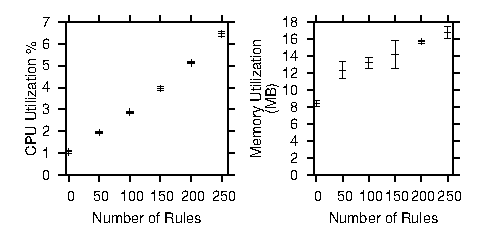
\includegraphics{newResults/manyJoins1}}
\caption{CPU and memory utilization (average, standard deviation) for
  an increasing number of piggybacked rules on a preexisting
  periodic event with period 1 sec.}
\label{fig:manyJoins1}
\end{figure}


Next we evaluate the performance overhead of two usage examples from
Section~\ref{sec:applications}: proactive consistency probes and consistent
snapshots.
Figure~\ref{fig:proactiveConsistency} plots overhead measurements for
the proactive consistency probes, running at increasing rates ranging
from once every 32 sec to once every sec.  The ``None'' point on the $x$
axis denotes running Chord without the consistency probes.  The figure
indicates that memory consumption and messages transmitted grow linearly
with the rate of the probe.  CPU utilization, however, grows
superlinearly with the rate, as frequent probes (and their multiple
lookups) contend for cycles on the initiator and all nodes in the
testbed. 

\begin{figure}
\centerline{\includegraphics{newResults/proactiveConsistency}}
\caption{CPU and memory utilization for the
  proactive inconsistency detector, with a rate
  (i.e., frequency of initiation) of $1/32$ to 1
  sec, alongside Chord without the detector (far
  left).}
\label{fig:proactiveConsistency}
\end{figure}


Figure~\ref{fig:snapshots} similarly plots the overheads caused by
consistent snapshots taken at rates from $1/32$ to $1$ snapshot per sec.
Linear growth of memory consumption is much  lower than with consistency
probes, and so is the superlinear rate at which CPU utilization grows.
Note, however, that consistent snapshots are much less taxing on the
system than the many parallel lookups initiated by consistency probes
for the same rates. Note also that the high rates that we measure here for
consistency probes and consistent snapshots are
for evaluation purposes; usually an operator would take snapshots at
much lower rates than these.
\begin{figure}
\centerline{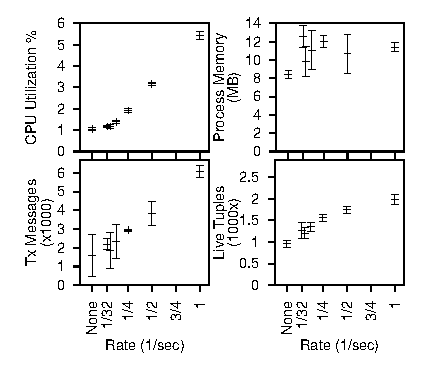
\includegraphics{newResults/snapshots}}
\caption{Consistent snapshots}
\label{fig:snapshots}
\end{figure}

\eat{

Finally, we measure the execution tracing example from
Section~\ref{sec:examples:profiling}.  For this experiment, we employ a
network emulation testbed (Emulab~\cite{emulab:website}).  We run 5
Chord nodes on every physical Emulab node, to a total of 50 physical and
250 virtual nodes.  Nodes are interconnected in a network emulating a
transit-stub topology with X\% msec transit-to-transit and Y\% msec
transit-to-stub latencies.  We run Chord over 1 hour, issuing lookups
from a single node every 5 sec, and profiling the execution of every
lookup.  We only measure overheads on the monitoring
node. Figure~\ref{fig:profiling} shows the results.
\begin{figure}
\centerline{\includegraphics{newResults/proactiveConsistency}}
\caption{Execution tracing.}
\label{fig:profiling}
\end{figure}
}



%%%%%%%%%%%%%%%%%%%%%%%%%%%%%%%%%%%%%%%%%%
\section{Related Work}
\label{sec:related}

Finding faults (bugs, anomalies, etc.) in networked systems is a large
and burgeoning field.  We limit ourselves here to representative
examples of specific related areas to provide a context for our work. 

{\bf Monitoring and debugging with databases.}
Management interfaces to networked systems often have a more-or-less
relational flavor, and database techniques have been used to
externally monitor, debug, and manage distributed
systems~\cite{conradie-sdne,Hy+,snodgrass-tocs,wolfson-ieee91}.
Logs are typically stored in centralized or clustered databases, and
subsequently queried.  \Sys takes a different approach: the query
processor is deeply embedded in the system, and has access to much more
detailed data on execution in realtime. 

{\bf Performance debugging. }
Recent
work~\cite{blackbox-sosp03,magpie-osdi04,causeway-hotos05,chen-path-04} 
provides mechanisms to profile existing networked systems on-line.
These approaches track the life cycle of events
as they pass through different system components (e.g., an HTTP
request causing a disk access, a page fault, etc.); the
information  gathered is then mined to find performance anomalies or
bottlenecks in the system.  Much of the achievement of these systems is
reconstructing meaningful data- and control-flow from low level
monitoring information.  \Sys avoids this challenge by constructing
the system in the first place such that high-level structural
information is retained and can be related to low-level tracing in a
natural way on-line by the query processor.  

{\bf Debugging configurations or intrusions.}
Several systems trace implications of configuration
errors by inferring causality
relationships~\cite{mahajan-sigcomm02,wang-osdi04,King2003}
or 
mining for events correlated with changes in system
behavior~\cite{chronus-osdi04}. Kiciman and Subramanian~\cite{Kiciman_hotdep_2005} provide a
model that constitutes a diagnosable system in the
same context.  \Sys is narrower in scope in this respect: our
examples are at present rule-based tests and metrics using detailed
execution information and system reflection, rather than large-scale
statistical measures and machine-learning techniques.

{\bf Distributed debuggers.}
\if 0
Garcia-Molina et al.~\cite{molina-tose} proposed debugging individual modules
independently before integrating and using tracing (logging) for debugging 
distributed systems. {\bf XXX: Could not get a copy of this on-line - Atul}
\fi
Early work by Bates et~al.~\cite{bates-83} proposed a high-level debugger
that compares the expected behavior of a network to the observed
behavior of the implementation.  The 
challenge lies in inferring system behavior from
observable information.  In \Sys, the high-level specification
of the system facilitates this by making explicit
the preconditions and expected output of each algorithmic step.

Harris~\cite{harris-EW02} proposed sandboxing
distributed components in a virtual machine monitor (VMM) to capture and
replay external factors affecting system execution
(e.g., processor status, scheduling, etc.).  We achieve something
close to this on-line by logging and analyzing the system's execution,
since we can observe the system at a level of abstraction
higher than processor flags and interrupts.

Closest to our vision is work by Lin et al.~\cite{wids-hotos05} on an
integrated toolkit for optimizing the implementation and testing of
distributed systems. The authors plan to generate
code from a high level specification that can run in both
simulation and real networks.  It is not yet clear what
high-level abstraction they will use.  In \Sys, we
compile a logic language to a dataflow graph,
providing for on-line debugging of the system at
multiple abstraction levels.

Recently, Geels et al.~\cite{Geels2006} proposed a technique for 
debugging distributed systems by logging the execution of 
deployed systems and replaying them deterministically for offline analysis. It 
also integrates \textit{gdb} to allow source level debugging. However, due
to its inherent requirement of replay at one site, it needs to ship logs to 
one place which is costly. Secondly, this technique is designed to find
non-deterministic bugs or race conditions, rather than violations of high-level 
correctness conditions.


Pip~\cite{pip_nsdi_2006} is a new methodology 
for debugging distributed systems. It works by comparing actual behavior and 
expected behavior to expose bugs. Programmers express expectations about a system's
structure, timing and other properties. Pip logs actual behavior and provides query and
visual interface for exploring the expected and unexpected behavior. It has been
shown to be useful in finding bugs in existing systems. However, Pip debugging
happens at a central place where all the system logs are collected and it is offline.

{\bf Debugging Languages.} Crawford et al.~\cite{Crawford1995} present a
framework for the design of imperative debugging
languages.  They construct a generic debugging
language, GDL, to capture the main required features for any
such language.  Many of the inspectional language
constructs of GDL are present in OverLog, although we do not yet
provide support for program \emph{control} such as stepping or
breakpointing.  It is unclear what the implications
of this might be
in an on-line networked environment. 

{\bf Deep embedded monitoring.} IBM Websphere XD provides a health monitoring 
subsystem for the IBM Websphere~\cite{IBM_web:website}. A set of rules or 
conditions are provided
which define the good health of the system. 
These conditions are monitored and
certain actions are taken when these conditions are
violated. For example, if memory usage of
an application hovers above the specified threshold for some specified 
period, an event may trigger the restart the
application.  Similarly, if a server is overloaded for a specified period of time, some of its work is offloaded to an underloaded server.
Typically, the conditions are performance oriented and lack the functional 
aspect of debugging (e.g., backtracking the causality chain to find the cause) as supported by our system.

Hollingsworth et al.~\cite{Hollingsworth_sc_1995} provides a mechanism for performance
monitoring of parallel programs by guiding the search of bottlenecks in
the program execution. It tries to answer three questions: why, where
and when does the bottleneck appear. The system starts with a given
set of hypotheses (e.g., synchronization is the bottleneck) provided by the user and depending
on the execution, a hypothesis is tested and automatically refined. This helps 
in reducing the trace data to be collected and at the same time zoom to the specific
area plagued by bottlenecks. The application needs to be recompiled to enable
instrumentation at appropriate places. The focus of this work is to find only the performance 
bottlenecks, however we focus on finding arbitrary
bugs and their root causes without need for recompilation.

Huang et al.~\cite{Huang_hpdc_2005} propose an architecture for adapting
applications to changing runtime environments using the event-action
based rules provided by the application designers. These event-action
rules explain what event to monitor and what action to take when that
particular event happens. This paper explains the difficulty in
building an architecture which can support this feature, as there
might be different adaptations which might conflict with each other,
both in terms of action as well as intent and how to identify these
conflicts and resolve them. Our work does not focus
on adaptations but on finding problems and their causes.

%%%%%%%%%%%%%%%%%%%%%%%%%%%%%%%%%%%%%%%%%%
\section{Conclusions}
\label{sec:conclusion}

The objective of this paper has been to argue that combining features of
``diagnosable'' systems, such as exposed state and execution
transparency, with features of ``diagnostic'' systems, such as the
ability to process distributed queries, it is possible to build
distributed systems that evolve along with their fault-finding tasks in
an organic and natural way.  We have proposed a candidate system based
on P2 that combines declarative query processing, execution logging,
and on-line execution tracing.  Finally, we have demonstrated and
measured the performance of a broad range of fault-finding tasks, both
local and distributed in scope, some simple and others as sophisticated
as complex distributed algorithms, to explore the power and flexibility
of our approach.

Many challenges remain ahead for our work.  We have extended our
execution logging facilities to the high-level declarative rule-based
execution abstraction of OverLog, the logic language in which P2
applications are specified.  However, faults can frequently be found
at lower-level abstractions, such as the dataflow graph abstraction on
which P2 applications are executed in practice.  Extending the language
to enable diagnostic specifications at lower-level abstractions is work
in progress and may inch away from the current logic language.
Furthermore, unlike rule-level diagnostics, dataflow-level diagnostics
must be specified with regards to a ``moving target'' lower
representation, which may be subject to transparent
optimizations.  Exposing useful state for diagnosis while still allowing
optimization clearly requires careful engineering.

Perhaps more importantly, this work will have to face a grander
challenge of scope.  Beyond the mechanistic applications we have
described here, fault finding typically extends to the very large
(anomaly detection in large distributed populations), the very small
(scheduling decisions or timing issues), and
the very complex
(intrusion detection and misbehavior).  P2's query-processing pedigree
suggests that large-scale statistical processing may be possible.
Prioritized execution of debugging rules may allow the unperturbed observation of
sensitive, low-level scheduling artifacts.  And the fine-grained
dataflow element building blocks of P2 may lend themselves well to
verifiable audit trails that can be inspected for undeniable
inconsistencies leading to detection of misbehavior.  Pursuing all of
these exciting possibilities is the subject of our
on-going work.


\section{Acknowledgments}
We would like to thank our shepherd Karsten Schwan and the anonymous
reviewers for their comments and suggestions.  We are also indebted to
Boon Thau Loo and Tyson Condie for their help with the P2 codebase and
experimental harness, as well as Joseph M. Hellerstein and
Lakshminarayanan Subramanian for their thoughtful comments on drafts of
this paper.


\bibliographystyle{abbrv}
\bibliography{debugging}

\eat{

\appendix

\section{Chord in \Lang}
\label{sec:chordOverlog}

Here we provide the full \Lang specification for Chord. This
specification deals with lookups, ring maintenance with a fixed number
of successors, finger-table maintenance and opportunistic finger table
population, joins, stabilization, and node failure detection.

\begin{overlog}
/* The base tuples */

materialize(node, infinity, 1, keys(1)).
materialize(finger, 180, 160, keys(2)).
materialize(bestSucc, infinity, 1, keys(1)).
materialize(succDist, 10, 100, keys(2)).
materialize(succ, 10, 100, keys(2)).
materialize(pred, infinity, 100, keys(1)).
materialize(succCount, infinity, 1, keys(1)).
materialize(join, 10, 5, keys(1)).
materialize(landmark, infinity, 1, keys(1)).
materialize(fFix, infinity, 160, keys(2)).  
materialize(nextFingerFix, infinity, 1, keys(1)).  
materialize(pingNode, 10, infinity, keys(2)).  
materialize(pendingPing, 10, infinity, keys(2)).  


/** Lookups */

L1 lookupResults@R(R,K,S,SI,E) :- node@NI(NI,N),
  lookup@NI(NI,K,R,E), bestSucc@NI(NI,S,SI), K in
  (N,S].
L2 bestLookupDist@NI(NI,K,R,E,min<D>) :-
  node@NI(NI,N), lookup@NI(NI,K,R,E),
  finger@NI(NI,I,B,BI), D:=K - B - 1, B in (N,K).
L3 lookup@BI(min<BI>,K,R,E) :- node@NI(NI,N),
  bestLookupDist@NI(NI,K,R,E,D),
  finger@NI(NI,I,B,BI), D == K - B - 1, B in (N,K).


/** Neighbor Selection */

N1 succEvent@NI(NI,S,SI) :- succ@NI(NI,S,SI).
N2 succDist@NI(NI,S,D) :- node@NI(NI,N),
  succEvent@NI(NI,S,SI), D:=S - N - 1.
N3 bestSuccDist@NI(NI,min<D>) :-
  succDist@NI(NI,S,D).
N4 bestSucc@NI(NI,S,SI) :- succ@NI(NI,S,SI),
  bestSuccDist@NI(NI,D), node@NI(NI,N), D == S - N
  - 1.
N5 finger@NI(NI,0,S,SI) :- bestSucc@NI(NI,S,SI).


/** Successor eviction */

S1 succCount@NI(NI,count<*>) :- succ@NI(NI,S,SI).
S2 evictSucc@NI(NI) :- succCount@NI(NI,C), C > 4.
S3 maxSuccDist@NI(NI,max<D>) :- succ@NI(NI,S,SI),
  node@NI(NI,N), evictSucc@NI(NI), D:=S - N - 1.
S4 delete succ@NI(NI,S,SI) :- node@NI(NI,N),
  succ@NI(NI,S,SI), maxSuccDist@NI(NI,D), D == S -
  N - 1.

/** Finger fixing */

F0 nextFingerFix@NI(NI, 0).
F1 fFix@NI(NI,E,I) :- periodic@NI(NI,E,10),
  nextFingerFix@NI(NI,I).
F2 fFixEvent@NI(NI,E,I) :- fFix@NI(NI,E,I).
F3 lookup@NI(NI,K,NI,E) :- fFixEvent@NI(NI,E,I),
  node@NI(NI,N), K:=1I << I + N.
F4 eagerFinger@NI(NI,I,B,BI) :- fFix@NI(NI,E,I),
  lookupResults@NI(NI,K,B,BI,E).
F5 finger@NI(NI,I,B,BI) :-
  eagerFinger@NI(NI,I,B,BI).
F6 eagerFinger@NI(NI,I,B,BI) :- node@NI(NI,N),
  eagerFinger@NI(NI,I1,B,BI), I:=I1 + 1, K:=1I << I
  + N, K in (N,B), BI != NI.
F7 delete fFix@NI(NI,E,I1) :-
  eagerFinger@NI(NI,I,B,BI), fFix@NI(NI,E,I1), I >
  0, I1 == I - 1.
F8 nextFingerFix@NI(NI,0) :-
  eagerFinger@NI(NI,I,B,BI), ((I == 159) || (BI ==
  NI)).
F9 nextFingerFix@NI(NI,I) :- node@NI(NI,N),
  eagerFinger@NI(NI,I1,B,BI), I:=I1 + 1, K:=1I << I
  + N, K in (B,N), NI != BI.


/** Churn Handling */

C1 joinEvent@NI(NI,E) :- join@NI(NI,E).
C2 joinReq@LI(LI,N,NI,E) :- joinEvent@NI(NI,E),
  node@NI(NI,N), landmark@NI(NI,LI), LI != "-".
C3 succ@NI(NI,N,NI) :- landmark@NI(NI,LI),
  joinEvent@NI(NI,E), node@NI(NI,N), LI == "-".
C4 lookup@LI(LI,N,NI,E) :- joinReq@LI(LI,N,NI,E).
C5 succ@NI(NI,S,SI) :- join@NI(NI,E),
  lookupResults@NI(NI,K,S,SI,E).


/** Stabilization */

SB0 pred@NI(NI,"-","-").
SB1 stabilize@NI(NI,E) :- periodic@NI(NI,E,15).
SB2 stabilizeRequest@SI(SI,NI) :-
  stabilize@NI(NI,E), bestSucc@NI(NI,S,SI).
SB3 sendPredecessor@PI1(PI1,P,PI) :-
  stabilizeRequest@NI(NI,PI1), pred@NI(NI,P,PI), PI
  != "-".
SB4 succ@NI(NI,P,PI) :- node@NI(NI,N),
  sendPredecessor@NI(NI,P,PI),
  bestSucc@NI(NI,S,SI), P in (N,S).
SB5 sendSuccessors@SI(SI,NI) :- stabilize@NI(NI,E),
  succ@NI(NI,S,SI).
SB6 returnSuccessor@PI(PI,S,SI) :-
  sendSuccessors@NI(NI,PI), succ@NI(NI,S,SI).
SB7 succ@NI(NI,S,SI) :-
  returnSuccessor@NI(NI,S,SI).
SB7 notifyPredecessor@SI(SI,N,NI) :-
  stabilize@NI(NI,E), node@NI(NI,N),
  succ@NI(NI,S,SI).
SB8 pred@NI(NI,P,PI) :- node@NI(NI,N),
  notifyPredecessor@NI(NI,P,PI),
  pred@NI(NI,P1,PI1), ((PI1 == "-") || (P in
  (P1,N))).


/** Connectivity Monitoring */

CM0 pingEvent@NI(NI,E) :- periodic@NI(NI,E,5).
CM1 pendingPing@NI(NI,PI,E) :- pingEvent@NI(NI,E),
  pingNode@NI(NI,PI).
CM2 pingReq@PI(PI,NI,E) :- pendingPing@NI(NI,PI,E).
CM3 delete pendingPing@NI(NI,PI,E) :-
  pingResp@NI(NI,PI,E).
CM4 pingResp@RI(RI,NI,E) :- pingReq@NI(NI,RI,E).
CM5 pingNode@NI(NI,SI) :- succ@NI(NI,S,SI), SI !=
  NI.
CM6 pingNode@NI(NI,PI) :- pred@NI(NI,P,PI), PI !=
  NI, PI != "-".
CM7 succ@NI(NI,S,SI) :- succ@NI(NI,S,SI),
  pingResp@NI(NI,SI,E).
CM8 pred@NI(NI,P,PI) :- pred@NI(NI,P,PI),
  pingResp@NI(NI,PI,E).
CM9 pred@NI(NI,"-","-") :- pingEvent@NI(NI,E),
  pendingPing@NI(NI,PI,E), pred@NI(NI,P,PI).

\end{overlog}



\section{Examples that might have been}

\subsection{***Inventory***}

What we have (or might have)

The dones:
\begin{itemize}
\item Consistent routing (successor in-degree, ring ordering, table
oscillation, proactive regression test, degree distribution)
\item Partition detection (ID density checks, reintegration checks)
\item Execution analysis (Profiling of running lookups)
\item Generic tools (pickling, consistent snapshots, regression tests)
\end{itemize}

The undones:
\begin{itemize}
\item Exhaustive causal classification of invariant violations
\item A distributed join of some sort (dead node visibility)
\item ID density checks at lookup source/destination as heuristic of
vulnerability.
\item Annotation of history with ``interesting'' or ``not interesting'' mark
according to information maximization criteria.
\item Condition timing / transience.
\end{itemize}


\subsubsection{Degree Distribution Over Snapshot. Remove?}
To illustrate the use of consistent snapshots in
understanding overlay properties, we provide an
example that computes the overlay degree
distribution on a consistent
snapshot.  The request is
flooded over the overlay links.  Each recipient 
computes its degree and sends it back 
to the requester.  Instead of sending the degree
directly, slightly more involved OverLog rules could
perform in-network aggregation, which we omit here for
brevity.
\begin{overlog}
dh1 degreeTok@NAddr(SnapID, E, NAddr) :-
   degreeEv@NAddr(SnapID, E).

dh2 seenBeforeToks@NAddr(SnapID, E, SrcAddr, count<*>)
   :- degreeTok@NAddr(SnapID, E, SrcAddr),
   pastDegreeToks@NAddr(E).

dh3 getDegree@NAddr(SnapID, E, SrcAddr) :-
   seenBeforeToks@NAddr(SnapID, E, SrcAddr, 0),

dh4 degreeTok@NAddr(SnapID, E, SrcAddr) :-
   getDegree@NAddr(SnapID, E, SrcAddr),
   pingNode@NAddr(NeighborAddr).

dh5 pastDegreeToks@NAddr(E) :- getDegree@NAddr(SnapID,
   E, SrcAddr).

dh6 degree@SrcAddr("" + SnapID + E, SnapID, E, NAddr,
   count<*>) :- getDegree@NAddr(SnapID, E, SrcAddr),
   snapFingers@NAddr(RecID, SnapID, FPos, FAddr, FID).

dh7 degreeHist@NAddr("" + Degree + DegreeID, DegreeID,
   Degree, count<*>) :- degree@NAddr(DegreeID, SnapID,
   E, SrcAddr, Degree).
\end{overlog}
Rules \ol{dh1} through \ol{dh5} flood the request.
Seen requests are stored in \ol{seenBeforeToks}, to
avoid duplicate request forwarding.  Rule \ol{dh6}
computes its degree over the fingers stored in the
named consistent snapshot, sending it back to the
requester.  Rule \ol{dh7} aggregates by degree to
compute the histogram \ol{degreeHist} for the given
degree request.



\subsection{Partition Detection}
\label{sec:examples:partitions}

Network partitions can wreak havoc in overlays.  Typically transient IP
routing faults cause the population to split into two subsets, in which
nodes within the same subset can communicate but no communication can
happen across subsets.  In more complex fault conditions, a pair of
nodes may lose direct connectivity while they can still communicate over
multiple application-level hops.  Sometimes havoc can persist after the
partition has passed, because the partitioned population subsets may
have partially separated during disconnection.

In this section we develop detectors for network partitions within the
Chord population, as well as for correct reintegration after the network
partition has passed.





assumption: overlay partition occurs due to temporal network partition, not due to node failure,
so most nodes are up and running but can not talk for the duration of 
partition.

Our case: For detection, do what FreePastry does. Monitor the density of nodes in
my nodeId vicinity and if it falls below 50\%, detect a partition. Currently, FreePastry
suggests that if I detect such a partition, I resign from the overlay and join again later.

Basic idea for Healing: if node A detects node B to be alive
and running the overlay app but does not find B in its overlay. To gain more faith, A
can obtain B's neighbors and do the checking for them in similar way. If this holds,
overlay could not recover and there are multiple overlays in existence. For this to 
work, A keeps a list of nodes that it detected dead (they didnt respond to pings) and 
pings them at exponential delayed times. 

Question: who does this checking? Is A a node in major partition or minor? Also,
how to distributed the load of this checking? Can we somehow use the identifier relations
such as A checks B only if A shares some digits with B?


\subsubsection{Single node identity density check}
Identity density is the average identity space distance between adjacent
successors of a node.

\begin{overlog}
d1 densityEvent@NAddr(NAddr) :- periodic@NAddr(NAddr,
   E, tCheck).

d2 densityExtent@NAddr(NAddr, max<D>) :-
   densityCheck@NAddr(NAddr, E), node@NAddr(NAddr,
   NID), succ@NAddr(NAddr, SID, SAddr), Dist := SID -
   NID - 1.

d3 density@NAddr(NAddr, Time, Density) :-
   densityExtent@NAddr(NAddr, E, Distance),
   succCount@NAddr(NAddr, Count), Density := Distance
   / (Count + 1), Time := now.
\end{overlog}


\subsubsection{Time series of density check}
Store the density. When new estimate arrives, compare to old density and
raise alarm if there's a big difference.  Rule \ol{nd1} pulls together
the last measured density and the newly measured density.  Rule \ol{nd2}
raises an alarm if the newly measured density is less than half the old
one.  Rule \ol{nd3} replaces the old logged density with the newly
measured one.

\begin{overlog}
materialize(densityLog, infinity, 1, keys(2)).

nd1 cmpDensities@NAddr(NAddr, NewTime, NewDensity,
   Density) :- density@NAddr(NAddr, NewTime,
   NewDensity), densityLog@NAddr(NAddr,Time,
   Density).

nd2 densityAlarm@NAddr(NAddr, Time, Density,
   OldDensity) :- cmpDensities@NAddr(NAddr, Time,
   Density, OldDensity), Density < OldDensity / 2.

nd3 densityLog@NAddr(Time, Density) :-
   cmpDensities@NAddr(NAddr, Time, Density,
   OldDensity).
\end{overlog}

Slightly more complex rules can check the new density over the average
of a sliding window.




\subsubsection{Reintegration checks}

Keep track of nodes that I've declared unresponsive.  If they become
responsive again, check that I can reach them via the overlay.

The overlay issues the \ol{unresponsive@NAddr(NAddr, NbrAddr)} event
when a neighbor \ol{NbrAddr} is detected as unresponsive.  We can do the
following to check the reintegration correctness of the system.
\begin{overlog}
materialize(secondChance, 1800, infinity, keys(2)).

materialize(reintroCheck, 60, infinity, keys(2,3,4)).

PU1 secondChance@NAddr(NAddr, NbrAddr) :-
   unresponsive@NAddr(NAddr,NbrAddr).

PU2 probeEv@NAddr(NAddr) :- periodic@NAddr(NAddr, E,
   tProbeUnresponsive).

PU3 identify@NbrAddr(NbrAddr, NAddr) :-
   probeEv@NAddr(NAddr), secondChance@NAddr(NAddr,
   NbrAddr).

PU4 identified@NbrAddr(NbrAddr, NAddr, NID) :-
   identify@NAddr(NAddr, NbrAddr), node@NAddr(NAddr,
   NID).

PU5 reintroCheck@NAddr(NAddr, NbrAddr, NbrID, E, T)
   :- identified@NAddr(NAddr, NbrAddr, NbrID),
   unresponsive@NAddr(NAddr,NbrAddr), E :=
   f_random(), T := now.

PU6 lookup@NAddr(NAddr, NID, NAddr, E) :-
   reintroCheck@NAddr(NAddr, NbrAddr, NbrID, E, T).

PU7 reintegrated@NAddr(NAddr, NbrAddr, NbrID) :-
   response@NAddr(NAddr, NbrID, NbrAddr, NbrID, E),
   reintroCheck@NAddr(NAddr, NbrAddr, NbrID, E, T).

PU8 partitioned@NAddr(NAddr, NbrAddr, NbrID) :-
   response@NAddr(NAddr,Key, SAddr, SID, E),
   reintroCheck@NAddr(NAddr, NbrAddr, NbrID,E, T),
   NbrAddr != SAddr.
\end{overlog}










\subsubsection{Pickling (Petros)}

Goal: intelligently pick ``interesting'' bits of state or history to
store persistently for further perusal.

Implementation: When an invariant violation is detected, walk backwards
the execution history of the invariant violation and copy the relevant
facts from the ring-buffered execution traces to instance-specific
non-expiring entries.

\begin{overlog}
materialize(pickledExec,infinity,infinity,key(1,3,4,5)).

t1 trace@NI(Out,Depth,ID) :-
   exec@NI(Rule,In,Out,Time), Depth :=10, Rule == r1,
   ID := f_random().

t2 pickledExec@NI(ID, Depth, Rule, In, Tuple, Time)
   :- trace@NI(Tuple,Depth, ID), Depth >= 0,
   exec@NI(Rule, In, Tuple, Time).

t2 trace@SourceAddr(In, NewDepth, ID) :-
   pickledExec@NI(ID, Depth, Rule,In, Out, Time),
   SourceAddr := f_source(In), NewDepth := Depth - 1.
\end{overlog}

Then run queries on the persistant entries, even after the original
history records have expired.  For example, the following query sends to
a designated node all precoditions of the violation with an age greater
than 10 sec.

\begin{overlog}
t1 findOld@Designated(In) :- ID == idInQuestion,
   pickledExec@NI(ID, Depth, Rule, In, Out,Time),
   InAge := f_age(In), InAge > 10, Designated :=
   myNode.
\end{overlog}

A more sophisticated example with consistent snapshots follows.


\subsubsection{Refinement}
Goal: find those bits of the execution history of an invariant violation
(e.g., the inconsistent routing task) that are likely to be contributing
causes.  Use the heuristic that an event is a likely contributor if it
is solely a precondition of invariant violations and does not appear in
the causal history of satisfied invariants.

Implementation: within a consistency probe, traverse backwards the
execution histories of all results, both correct and incorrect.  Mark
each precondition traversed as ``correct'' if it appears in the
execution graph of a correct result or ``incorrect'' if it appears in
the execution graph of an incorrect result.  Filter out preconditions
that are marked ``correct'' or both ``correct'' and ``incorrect.''




\subsubsection{Lossy links or chaotic nodes (Later)}

Goal: detect part of the overlay graph where high losses occur or some
erratic nodes exist.

Nodes monitor the links and their loss rates. If this state is also maintained in table,
we can write queries which can check if every neighbor of a node is observing such a loss.
We can then disambiguate between erratic nodes or lossy links. These nodes or links could then
be avoided.



\subsubsection{Exhaustive Causal Classification (Later)}

High-level goal: which occuring routing inconsistencies are due to which
bug?

Typical implementation: Query detects a new inconsistency (as any
detector above), automatically traces the execution history of that
inconsistency (e.g., the causal graph of that particular inconsistency
10 causal hops back), and gives it to human.  Human can eyeball this
execution history of the inconsistency or query it more finely in place,
until human understands the bug (e.g., lookup was forwarded to dead
node) and writes a query that recognizes the occurrence of that bug
causing routing inconsistencies.  Human installs the recognizer in the
running system. Repeats, picking an inconsistency whose cause is not
recognized by any existing recognizer.

Over time, human can count how many inconsistencies occurred due to each
distinct bug identified thus far, can look at correlated occurrence of
different bugs causing inconsistencies, can look at spatial correlation
of bug occurrences among nodes in close topological proximity,
etc... Infinite options here.

Skip to next.



\subsubsection{Transience}
Goal: Find the duration of an invariant
violation (routing inconsistency) without point sampling.

Implementation: Once inconsistency is detected Detect condition, track
all necessary preconditions that make it true, track history to start
(last necessary but missing precondition became true) and to end (first
necessary precondition became false).  Characterize the transience of
complex distributed system states.


\subsubsection{Plugging Vulnerabilities in Insecure Overlays?}

Still in the conceptual stage.

This is our earlier ``shield'' idea.  Identify execution pattern that
might signify that Chord is being vulnerable and raise alarms.

Our thrust is: it's hard to build secure overlays. What if we just
resigned to using insecure overlays but built detectors of
vulnerability, either to shut down the offending session (request,
transaction, ...) or to log for subsequent reckoning.




\section{Longer related work}

Related work is split into three parts: first is on distributed monitoring, 
invariant checking and second is on distributed debuggers and third on the 
declarative specification.

\begin{itemize}

\item{\bf A relational approach to monitoring complex systems} Snodgrass~\cite{}present a 
relational database and query methods for monitoring distributed 
systems. It works in four stages. A user specifies the information to be collected 
via a specification language. System then instruments the codebase with the sensor 
code. User then submits the relational queries and monitor turns on the sensors 
which are needed to solve the queries. Final stage is the execution stage. Proposes 
TQuel (Temporal Quel) which incorporates the notion of \emph{time}. Also, 
makes operators \emph{incremental} so that they can operate on stream of 
tuples as they arrive. There are two problems with this work. First, they 
evaulated the system on a tightly coupled multiprocessor (Cm*, having 50 processors) 
with a centralized analysis component. Second, the authors present only 
microbenchmark results to demonstrate the feasibility of the approach and 
its not clear if they have actually used the system for actual monitoring.


Conradie~\cite{conradie-sdne} essentially follow the same principle of applying 
relational database ideas into distributed system management. This work builds 
up a management system, so users can request information via providing a relational 
query which are optimized and automatically dispersed in the network. Query 
evaluation happens in a distributed fashion, thereby making the approach scalable. 

\item{\bf Monitoring distributed systems} Joyce et. al~\cite{} present an 
infrastructure which supports the observation and control of the events 
(e.g., opening a file) occuring with respect to a process. The system monitors 
the full activity of the application processes which are being monitored in 
contrast to the relational approach where only query-specified information 
is collected. This paper focuses only on collecting such information, 
interpretation and processing is left as future work. Its design is not 
scalable as it contains centralized modules, e.g,. controllers which log all information.

\item{\bf HiFi} This paper~\cite{alshaer99hifishort} uses declarative language 
for specifying the monitoring requests and installs sensors in the system 
to detect and collect the required data. Uses hierarchical filters for 
scalability. Users subscribe for events for which they are interested in. 
Allows dynamic monitoring since the filters can be modified. Drawback is 
that their experimental evaluation is over a LAN. The major technical 
difference is that they use declarative langauage \emph{only} for specifiying 
the filters which affect the data which will be collected.


\item{\bf Monitoring databases for network management} Wolfson et. al~\cite{wolfson-ieee91} 
propose to manage communication networks by monitoring databases. Network 
management functions are specified as data manipulation statements. The 
database is continously updated to represent the current status of the network. 
Monitoring the network translates to watching for certain events to occur and 
in database, this converts to continous retrieval of this data-pattern. This 
paper provides new langugage features which allow real-time monitoring of 
database changes. Specifically, it allows the specification of correlated 
events and trace-collections which enable tracking the history of evolution 
of a particular attribute. They use RDL1 which is a rule-based langugage. 
Unfortunately, they leave the design of network database as future work.

\item{\bf Performance Assertion Checking and Continous monitoring} 
Perl and Weihl~\cite{perl-sosp93short} present an approach to automate the 
testing of performance properties of complex properties. The users 
specify the assertions in a high level language (PSpec) and these 
assertions are checked automatically with the monitored data (present in logs) 
to detect potential performance bugs. Note that the system is an offline 
verifier since it uses system logs to check what happend in the past. The 
evaulation suggests that the proposed system was able to find performance 
bugs in a parallel language. However, PSpec does not appear to have its 
ground in declarative languages and it is unclear if it is expressive enough.

Continous monitoring (CMon)~\cite{perl-cmon} is an extension to their 
above mentioned work. CMon provides the ability to capture logs produced 
by appropriately instrumented programs while the programs are being run 
by users, and direct the logs to apropriate processing programs.

\item{\bf Causeway} Appeared in HotOS this year. Basically, this system is 
used for metadata propagation, such as priority, in a distributed system. 
THe events are tagged with the metadata and when events traverse from one 
domain to another,the metadata is transferred from sending domain to receiving domain.


\item{\bf Magpie:} path taken by requests in a distributed system, can 
be used for capacity planning, performance debugging and anomaly detection.


\item{\bf Path-based failure and evolution management} This paper~\cite{chen-path-04} 
presents a new approach for detecting failures in complex distributed systems. The 
path taken by a request is the core abstraction provided by this paper, it 
records necessary information in sufficient volume to enable statistical 
analysis, failure detection is based on statistical deviation from expectation. 
However, the proposed solution is geared toward small sized system (a web server), 
logs the necessary information at a centralized repository and does not 
currently detect failure of distributed invariants.



\item{\bf Hy+:} Mariano et. al~\cite{Hy+} present a network management and 
distributed debugger based on declarative queries on collective data. They 
use the system for both network monitoring and debugging distributed systems.


\item{\bf WiDS:} Lin et. al~\cite{wids-hotos05} present an integrated toolkit 
for optimizing the process of implementation, testing and implementation of 
distributed systems. The emphasis of this work is ``code once, run many ways'', 
meaning that same code can run in simulation as well as real network, with 
added support for running extremely large simulations. However, they are 
still in research phase about replay facility and automating code 
generation ability from high level language. P2 already provides the 
second part. Also they utilize event driven model which makes debugging 
difficult. Data-flow model might help and make it easier.

\item{\bf Detecting causal relationships in distributed computations} 
Schwarz and Mattern~\cite{Schwarz94} show 

\item{\bf Consistent global snapshot}

\item{\bf Consistent detection of global predicates}  Cooper and Marzullo 91

\item{\bf Global events and global breakpoints in distributed systems} D Haban and W. Weigel 88

\item{\bf Modelling concurrency in parallel debugging} Hseush and Kaiser SIGPLAN 90

\item{\bf Optimal tracing and replay for debugging message-passing parallel programs} 
Netzer and Miller Suprecomputing 1992

\end{itemize} 



} %End of giant eat



\end{document}

% LocalWords:  dataflow DHT NetT LocalT LastT OutT RuleT InT ep ruleExec sr FID
% LocalWords:  FPos FAddr PAddr PID Src SAddr LookupID SrcSnapID MySnapID pred
% LocalWords:  SnapID snapState bestSucc snapBestSucc snapFingers snapPred NID
% LocalWords:  pingNode haveSnap backPointer lookupResults returnSuccessor
% LocalWords:  RespAddr ReqAddr rewriten NAddr SrcAddr ProbeID
